%!TEX TS-program = xelatex
%!TEX encoding = UTF-8 Unicode

% Load Thesis Class
\documentclass{DEIThesis}

\title{Reti neurali convoluzionali per lo studio di varianti non codificanti in sequenze genomiche}

\author{Alessandro Trigolo}
\studentId{2043049}

% Advisor
\advisor{Prof.ssa Cinzia Pizzi}

% If you are co-advised
\coadvisor{}

\university{Università degli Studi di Padova}
\mastername{Ingegneria Informatica}
\academicYear{2023/2024}

\begin{filecontents*}[overwrite]{\jobname.xmpdata}
    \Title{Reti neurali convoluzionali per lo studio di varianti non codificanti in sequenze genomiche}
    \Author{Alessandro Trigolo}
    \Language{it-IT}
    \Keywords{Computer Engineering\sep Bioinformatics\sep Convolutional Neural Networks\sep Non-coding variants \sep }
\end{filecontents*}


\setuptodonotes{fancyline, color=green!40, inline}

% Document

\begin{document}
    % The front matter (Cover, ToC, Abstract, etc...)
    \frontmatter

    % The main content
    \mainmatter
    
    %!TEX root = ../main.tex

\chapter{Introduzione}\label{chp:introduction}

Ad oggi l'avanzamento della genomica — ramo della biologia molecolare che si occupa di studiare il genoma degli esseri viventi — si è rivelato notevolmente significativo al fine di approfondire e comprendere malattie legate alle mutazioni del genoma degli individui. Si stima che solamente una percentuale tra l'1\% e il 2\% del \acs{DNA} contiene i \textsl{geni}, ovvero particolari regioni che contengono tutte le informazioni necessarie per la sintesi degli aminoacidi che poi comporranno le proteine\,\cite{sahu2011identification, pollard2022cell}. Ciò nonostante, la quasi totalità dei disturbi genomici è dovuta alle mutazioni nelle regioni non codificanti\,\cite{zhang2015non} — dette \textsl{varianti non codificanti}. Le mutazioni in queste zone del genoma, che apparentemente svolgono funzioni marginali, sono responsabili dello sviluppo di disturbi importanti, come le \textsl{malattie mendeliane}\footnote{Le malattie mendeliane, causate dalla mutazione di un singolo gene, includono la fibrosi cistica e il morbo di Huntington.}, l'epilessia, malattie cardiovascolari e soprattutto tumori — tra cui il cancro del colon-retto e il tumore al seno\,\cite{french2020role, chial2008mendelian, pagni2022non, kapoor2014enhancer, zhang2015non, khurana2016role, tian2019systematic, bojesen2013multiple, michailidou2017association}. Risulta quindi vitale continuare a studiare gli effetti che le varianti non codificanti in sequenze genomiche hanno sugli individui.

Negli ultimi decenni, il progredire delle tecniche di \textsl{sequenziamento}\,\cite{pareek2011sequencing} ha dato uno slancio rilevante allo sviluppo della \textsl{bioinformatica} — disciplina che unisce informatica e biologia. La bioinformatica si interessa a organizzare dati biologici in modo tale da facilitare l'accesso e l'inserimento di nuove informazioni (come il \acs{PDB}\,\cite{burley2017protein}), sviluppare \textsl{tool} che permettono l'analisi dei dati e infine fornire una interpretazione significativa dei risultati ottenuti\,\cite{luscombe2001bioinformatics}. Più recentemente, l'accrescimento dei dati biologici e il costante avanzamento della potenza di calcolo hanno reso possibile l'applicazione di tecniche di \textsl{deep learning} (\acs{DL}) anche nel campo della bioinformatica. Questo notevole progresso consente di scoprire e perfezionare soluzioni informatiche che permettano di delineare con sempre maggior precisione il ruolo che hanno le mutazioni nelle regioni non codificanti del \acs{DNA}.\@ Grazie a queste nuove tecnologie, la \textsl{genomica funzionale} — area della genomica che si interessa a descrivere le relazioni che ci sono tra i componenti di un sistema biologico, come geni e proteine\,\cite{caudai2021ai} — ha avuto un forte impulso nell'approfondire le varianti non codificanti, tuttavia rimangono ancora significative lacune nella comprensione della relazione tra mutazioni genetiche ed espressione genica. L'utilizzo di tecniche di deep learning risulta quindi cruciale per continuare la ricerca in questo ambito. L'obiettivo di questo elaborato è di discutere e confrontare tre tool che utilizzano le \textsl{reti neurali convoluzionali} per predire l'effetto delle varianti non codificanti su sequenze genomiche: DeepSEA\,\cite{zhou2015predicting}, Basset\,\cite{kelley2016basset} e DeepSATA\,\cite{ma2023deepsata}.

Più precisamente, il Capitolo\,\ref{chp:biological-background} introdurrà le basi della biologia molecolare, necessarie per comprendere interamente l'importanza delle varianti non codificanti. Successivamente, nel Capitolo\,\ref{chp:neural-networks} saranno approfonditi i principi fondamentali delle reti neurali e il modo in cui le reti convoluzionali possono essere utilizzate come ottimo strumento per predire l'effetto di sequenze genomiche. Il Capitolo\,\ref{chp:CNN-non-coding-variants} invece esaminerà i dettagli implementativi di ciascuno dei tre tool, indagando principalmente sugli aspetti legati alla codifica delle sequenze, alla struttura della rete e al \textsl{dataset} utilizzato per allenare il modello. Infine nel Capitolo\,\ref{chp:discussion} si riassumono le differenze analizzate nel capitolo precedente, offrendo una visione complessiva del confronto tra i tre tool.

% https://books.google.it/books?hl=it&lr=&id=Cg4WAgAAQBAJ&oi=fnd&pg=PP1&dq=Introduction+to+cell+biology&ots=yg4LdM46O3&sig=FkW8Ei_rOFccb96Sw3A28QsHuFo&redir_esc=y#v=onepage&q=Introduction%20to%20cell%20biology&f=false

% https://books.google.it/books?hl=it&lr=&id=mXiiEAAAQBAJ&oi=fnd&pg=PP1&dq=cellular+biology&ots=8O1TrOZBXp&sig=fqZhVnT0H-I3qEu1iPk4v2nvZi8&redir_esc=y#v=onepage&q=cellular%20biology&f=false

% https://books.google.it/books?hl=it&lr=&id=z4BDRcLrekMC&oi=fnd&pg=PR19&dq=cell+nucleus+organization&ots=wiXN8JbVpC&sig=oviVqMKJqsvcYwe4X37tQM28P3Y&redir_esc=y#v=onepage&q=cell%20nucleus%20organization&f=false

% Images:
% https://www.genome.gov/genetics-glossary

    %!TEX root = ../main.tex

\chapter{Background biologico}\label{chp:biological-background}

La cellula è l'unità fondamentale della vita. La cellula è una piccola miscela acquosa con componenti chimici, racchiusi in una membrana, e possiede l'eccezionale capacità di replicarsi. Il primo elemento che permette di distinguere le cellule è la presenza di un nucleo. Vengono definite \textsl{procarioti} le cellule senza nucleo — che sono le più diffuse e compongono organismi unicellulari come i batteri e gli archei — mentre sono chiamate \textsl{eucarioti} le cellule che contengono un nucleo — le quali sono in genere più grandi e più complesse e costituiscono forme di vita multicellulari come animali, piante e funghi\,\cite{alberts2015essential}.

All'interno della cellula eucariote (Figura\,\ref{fig:cell}), immersi nel \textsl{citoplasma}, sono presenti diversi \textsl{organuli}, i quali svolgono una particolare funzione ciascuno. I \textsl{mitocondri} sono gli organuli più diffusi.
% 
\begin{figure}[b!]
    \centering
    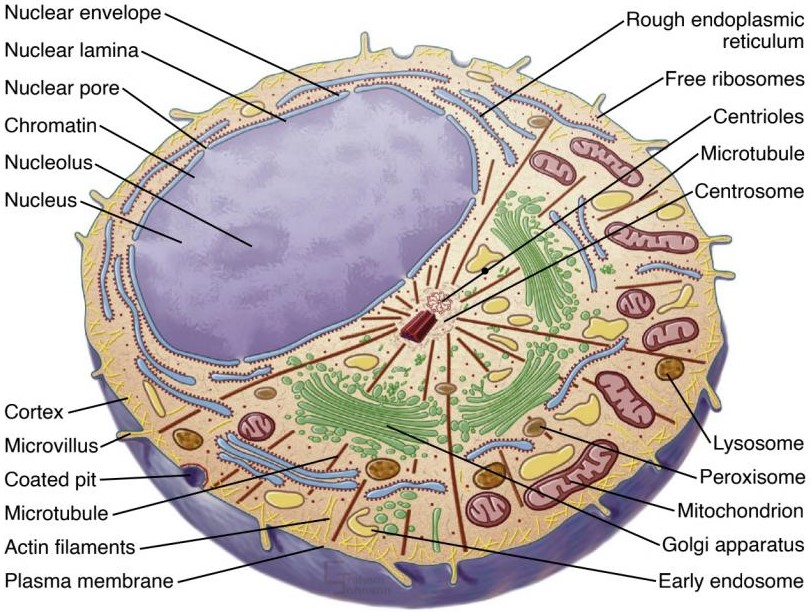
\includegraphics[width=.65\textwidth]{assets/cell.jpg}
    \caption[Rappresentazione schematica della cellula eucariote.]{Rappresentazione schematica della cellula eucariote; si possono notare i principali organuli tra cui i mitocondri, lisosomi e perossiomi, il reticolo endoplasmatico, e il nucleo\,\cite{pollard2022cell}.}\label{fig:cell}
\end{figure}
% 
Il loro compito è quello di generare energia chimica per la cellula: attraverso il processo di ossidazione di zuccheri e grassi, viene creata una sostanza che viene utilizzata nella maggior parte delle attività cellulari\footnote{Questa sostanza è detta \textsl{adenosintrifosfato} o ATP ed ha una struttura simile ad un nucleotide: è infatti composta dall'Adenina, da uno zucchero e da tre gruppi fosfati.}; questo processo è anche chiamato \textsl{respirazione cellulare} perché consumando l'ossigeno viene rilasciata anidride carbonica\,\cite{alberts2015essential, chinnery2003mitochondria}. Oltre ad essere la fonte energetica primaria della cellula, i mitocondri hanno anche importanti ruoli nella regolazione del metabolismo, del ciclo cellulare, delle risposte antivirali e anche della morte della cellula\,\cite{mcbride2006mitochondria}.

Il \textsl{reticolo endoplasmatico} è invece un organulo molto esteso e svolge molteplici funzioni. Tra questi compiti rientrano quelli di traslocazione di proteine e il ripiegamento delle proteine (\textsl{protein folding})\,\cite{alberts2015essential, voeltz2002structural}. I \textsl{lisosomi} si occupano di degradare e riciclare gli scarti cellulari e giocano un ruolo fondamentale per l'omeostasi della cellula\footnote{Con omeostasi cellulare si intende l'insieme di meccanismi necessari per mantenere ad un livello ottimale le funzioni della cellula.}, il suo sviluppo e il suo invecchiamento\,\cite{ballabio2016awesome, yang2021lysosome, dell2000lysosome}. Infine, i \textsl{perossiomi} sono delle piccole vescicole che forniscono un ambiente protetto per gestire molecole tossiche come gli acidi grassi i quali sono smaltiti tramite la $\beta$-ossidazione\,\cite{alberts2015essential, islinger2012peroxisome}.

L'organulo più importante della cellula rimane il \textsl{nucleo}. Racchiuso nell'\textsl{involucro nucleare}, all'interno di questo organulo sono presenti tutte le informazioni genetiche, racchiuse in una lunga molecola di acido desossiribonucleico (comunemente noto come DNA), che, una volta impacchettato forma il \textsl{cromosoma}\,\cite{pollard2022cell, alberts2015essential}. La molecola di DNA è una struttura a doppia elica formata da \textsl{nucleotidi}. Osservando la Figura\,\ref{fig:dna}, i nucleotidi sono composti a loro volta da tre elementi fondamentali: una \textsl{base azotata}, uno \textsl{zucchero} e un \textsl{gruppo fosfato}\footnote{I gruppi fosfati hanno una carica negativa e forniscono alla molecola le proprietà di un acido.}.
% 
\begin{figure}[b!]
    \centering
    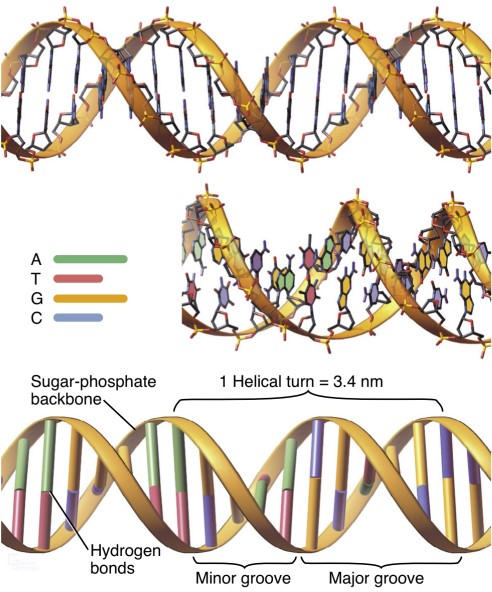
\includegraphics[width=\textwidth]{assets/dna.jpg}
    \caption[Rappresentazione schematica del DNA.]{Rappresentazione schematica del DNA in cui si possono osservare le coppie di basi azotate, legate tra loro attraverso gli zuccheri e i gruppi fosfati\,\cite{nhgri_dna_image}.}\label{fig:dna}
\end{figure}
% 
Le basi azotate sono quattro — Adenina (A), Citosina (C), Guanina (G) e Timina (T) — e si uniscono tra loro mediante dei legami ad idrogeno e secondo un preciso criterio: l'Adenina si lega solamente con la Timina (formando il legame \textit{AT}) mentre la Citosina si unisce solo con la Guanina (creando la coppia \textit{CG})\,\cite{fonseca2000hydrogen, sahu2011identification}. Si osserva infine che il nucleotide di una coppia e quello successivo si legano mediante zucchero e gruppo fosfato sempre allo stesso modo: il gruppo fosfato di un nucleotide si lega sempre allo zucchero dell'altro. Di conseguenza, preso un filamento della doppia elica, le due estremità non sono uguali in quanto una termina con un gruppo fosfato (terminazione $5^\prime$) e l'altra con uno zucchero (terminazione $3^\prime$).

Attraverso una serie di ripiegamenti, una molecola di DNA lunga circa due metri riesce a raggomitolarsi in un cromosoma di grandezza inferiore a 2 micron (Figura\,\ref{fig:dna-packaging}). Il processo di \textit{DNA-packaging} inizia avvolgendo la doppia elica di DNA attorno a delle proteine dette \textsl{istoni} e formando dei \textsl{nucleosomi}. In secondo luogo i nucleosomi si ammassano vicini tra loro formando una fibra, chiamata \textsl{cromatina} che, a sua volta si impacchetta su se stessa creando il cromosoma\,\cite{jansen2011nucleosome, zheng2010packaging}.

\begin{figure}[b!]
    \centering
    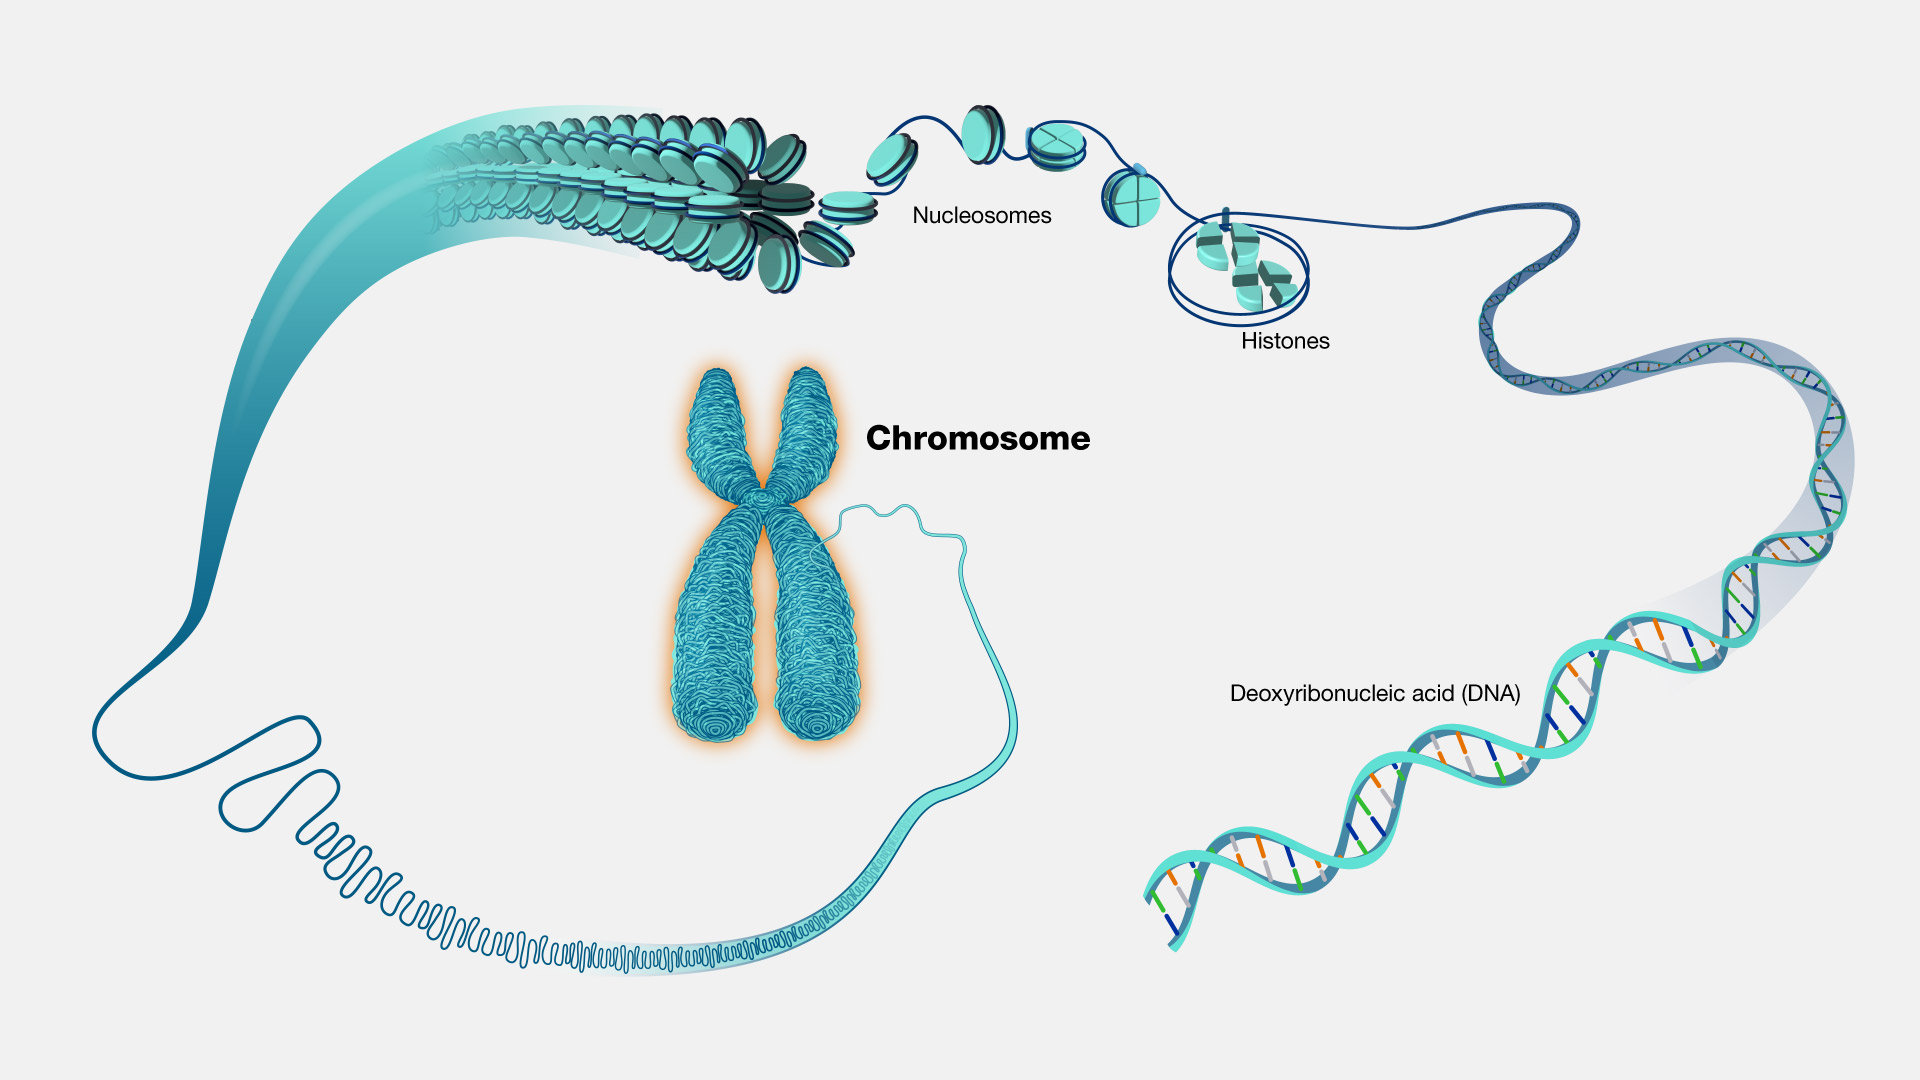
\includegraphics[width=\textwidth]{assets/dna-packaging.jpg}
    \caption[Il processo di impacchettamento del DNA.]{Il processo di impacchettamento del DNA che permette di compattare la struttura a doppia eilca nel cromosoma\,\cite{nhgri_chromosome_image}.}\label{fig:dna-packaging}
\end{figure}

\section{Dogma centrale}

La rilevanza del DNA è data delle informazioni essenziali che questa molecola contiene. Tali informazioni risiedono nei geni, che sono delle sequenze genomiche che codificano uno o più prodotti biologici operativi\,\cite{gerstein2007gene}. L'\textsl{espressione genica} è il processo che permette di utilizzare i dati contenuti nel gene per la creazione di macromolecole, come le proteine. Per esempio, le cellule della pelle a contatto con luce solare intensa possono esprimere geni che regolano la pigmentazione della pelle\,\cite{white2009gene}. L'espressione genica è divisa in due fasi principali: la \textsl{trascrizione} — che si occupa di produrre delle molecole di RNA che rispecchino il gene da esprimere — e la \textsl{traduzione} — la quale traduce le informazioni dell'RNA sintetizzando la proteina.

Nella prima fase dell'espressione genica, è necessario trascrivere il DNA in una molecola molto simile ovvero l'RNA — chiamato anche acido ribonucleico. Questa molecola differisce dall'acido desossiribonucleico per una base azotata — anziché la Timina è presente l'Uracile (U) — e per lo zucchero — da desossiribosio a ribosio\,\cite{alberts2002dna}. La trascrizione del DNA in RNA inizia quando delle proteine, chiamate \textsl{fattori di trascrizione}, attratte dagli \textit{enhancer} del DNA, riconoscono la regione che delimita l'inizio della molecola del gene da esprimere, detta \textsl{zona promotrice}. Dopo aver riconosciuto l'inizio della sequenza, queste proteine permettono ad un enzima chiamato \textsl{RNA polimerasi} di attaccarsi ed aprire la doppia elica del DNA\,\cite{cramer2019organization}. Una volta aperta la doppia elica, inizia la vera e propria trascrizione in RNA:\@ il filamento del DNA viene preso come modello per la creazione dell'RNA;\@ in particolare il nucleotide dell'RNA sarà il complementare rispetto a quello del DNA (di conseguenza $A\rightarrow U$, $C\rightarrow G$, $G\rightarrow C$ e $T\rightarrow A$). Così facendo l'acido ribonucleico viene creato un nucleotide alla volta, analizzando quello del DNA\,\cite{alberts2002dna}. La trascrizione termina nel momento in cui gli enzimi e le proteine incontrano la regione terminatrice del gene che determina la separazione dal filamento e la terminazione dell'RNA \textsl{messaggero} (\textsl{mRNA}) che contiene le informazioni presenti nel gene da esprimere. L'intero processo di trascrizione è illustrato nella Figura\,\ref{fig:dna-transcription}.

\begin{figure}[b!]
    \centering
    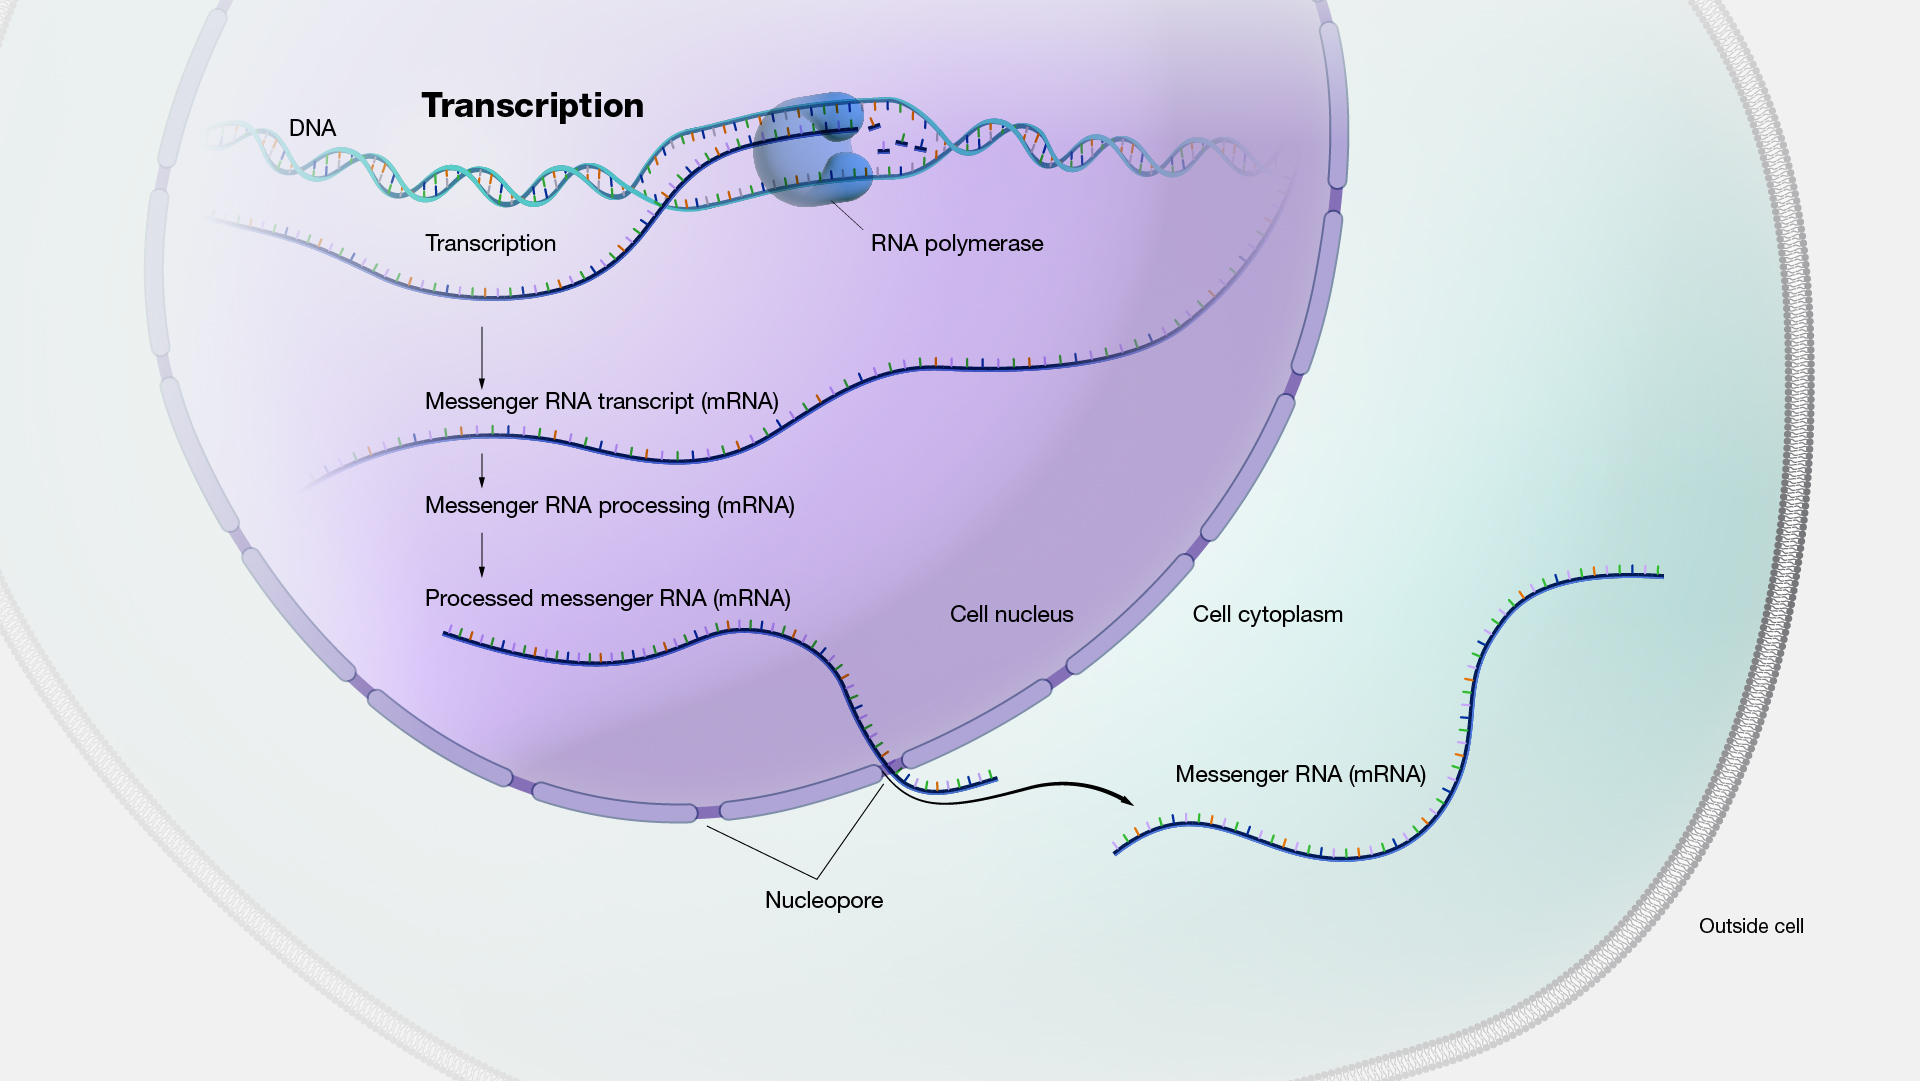
\includegraphics[width=\textwidth]{assets/dna-transcription.jpg}
    \caption[Il processo di trascrizione del DNA in RNA.]{Il processo di trascrizione del DNA del gene in RNA mediante la RNA polimerasi\,\cite{nhgri_transcription_image}.}\label{fig:dna-transcription}
\end{figure}

Prima di uscire dal nucleo l'RNA messaggero subisce una serie di elaborazioni necessarie per rendere le informazioni immagazzinare sicure: diverse sono le malattie che emergono per mutazioni presenti nell'mRNA tra cui la distrofia miotonica\footnote{Le distrofie miotoniche sono patologie che colpiscono principalmente l'apparato muscolo-scheletrico.}\,\cite{philips2000rna}. La prima elaborazione viene chiamata $5^\prime$-\textit{end capping} e si occupa di aggiungere alla terminazione $5^\prime$ dell'mRNA una Guanina attraverso un collegamento inusuale che garantisce maggiore stabilità alla molecola. In secondo luogo avviene lo \textit{splicing} che si occupa di rimuovere le zone non codificanti — dette \textsl{introni}— dal gene trascritto mantenendo solo quelle che verranno utilizzate per essere sintetizzate in proteine — gli \textsl{esoni} — e quindi facilitando il processo di traduzione. Infine con il $3^\prime$-\textit{end processing} viene aggiunta alla terminazione $3^\prime$ dell'mRNA una coda di Adenine — datta anche \textit{poly}A \textit{tail} — che, in maniera molto simile al $5^\prime$-\textit{end capping} garantisce una stabilità del filamento di acido ribonucleico\,\cite{hocine2010rna, livingstone2010mechanisms}.

Dopo essere uscito dal nucleo attraverso i \textsl{pori}, l'RNA messaggero raggiunge il citoplasma ed è pronto per iniziare la seconda fase dell'espressione genica, la traduzione. La traduzione non è altro che la traduzione dell'mRNA in un \textsl{polipeptide}, ovvero una sequenza di aminoacidi che compongono la proteina. Gli aminoacidi sono più di 20, di conseguenza anziché codificare un solo nucleotide dell'RNA messaggero, vengono codificati tre nucleotidi alla volta: questa tripletta viene chiamata \textsl{codone}. Durante la fase della traduzione, giocano un ruolo fondamentale i \textsl{ribosomi} i quali sono degli organuli nei quali avviene la traduzione. I ribosomi sono composti da due sotto unità, ciascuna delle quali ha tre siti per l'RNA di \textsl{trasporto} (\textsl{tRNA}). Delle due sotto unità del ribosoma, quella dimensionalmente minore si lega all'mRNA e agli \textsl{anticodoni} (sequenze specifiche di tre basi nel tRNA) e controlla che la traduzione avvenga con successo. La sotto unità più voluminosa invece si prende carico di catalizzare il legame peptidico tra l'aminoacido trasportato dal tRNA e la catena di aminoacidi in crescita\,\cite{ramakrishnan2002ribosome, lemonniermarathon, livingstone2010mechanisms}. In questo modo i ribosomi, analizzando codone dopo codone riescono a creare la catena polipeptidica mediante l'RNA di trasporto, come mostrato nella Figura\,\ref{fig:mrna-translation}.

\begin{figure}[b!]
    \centering
    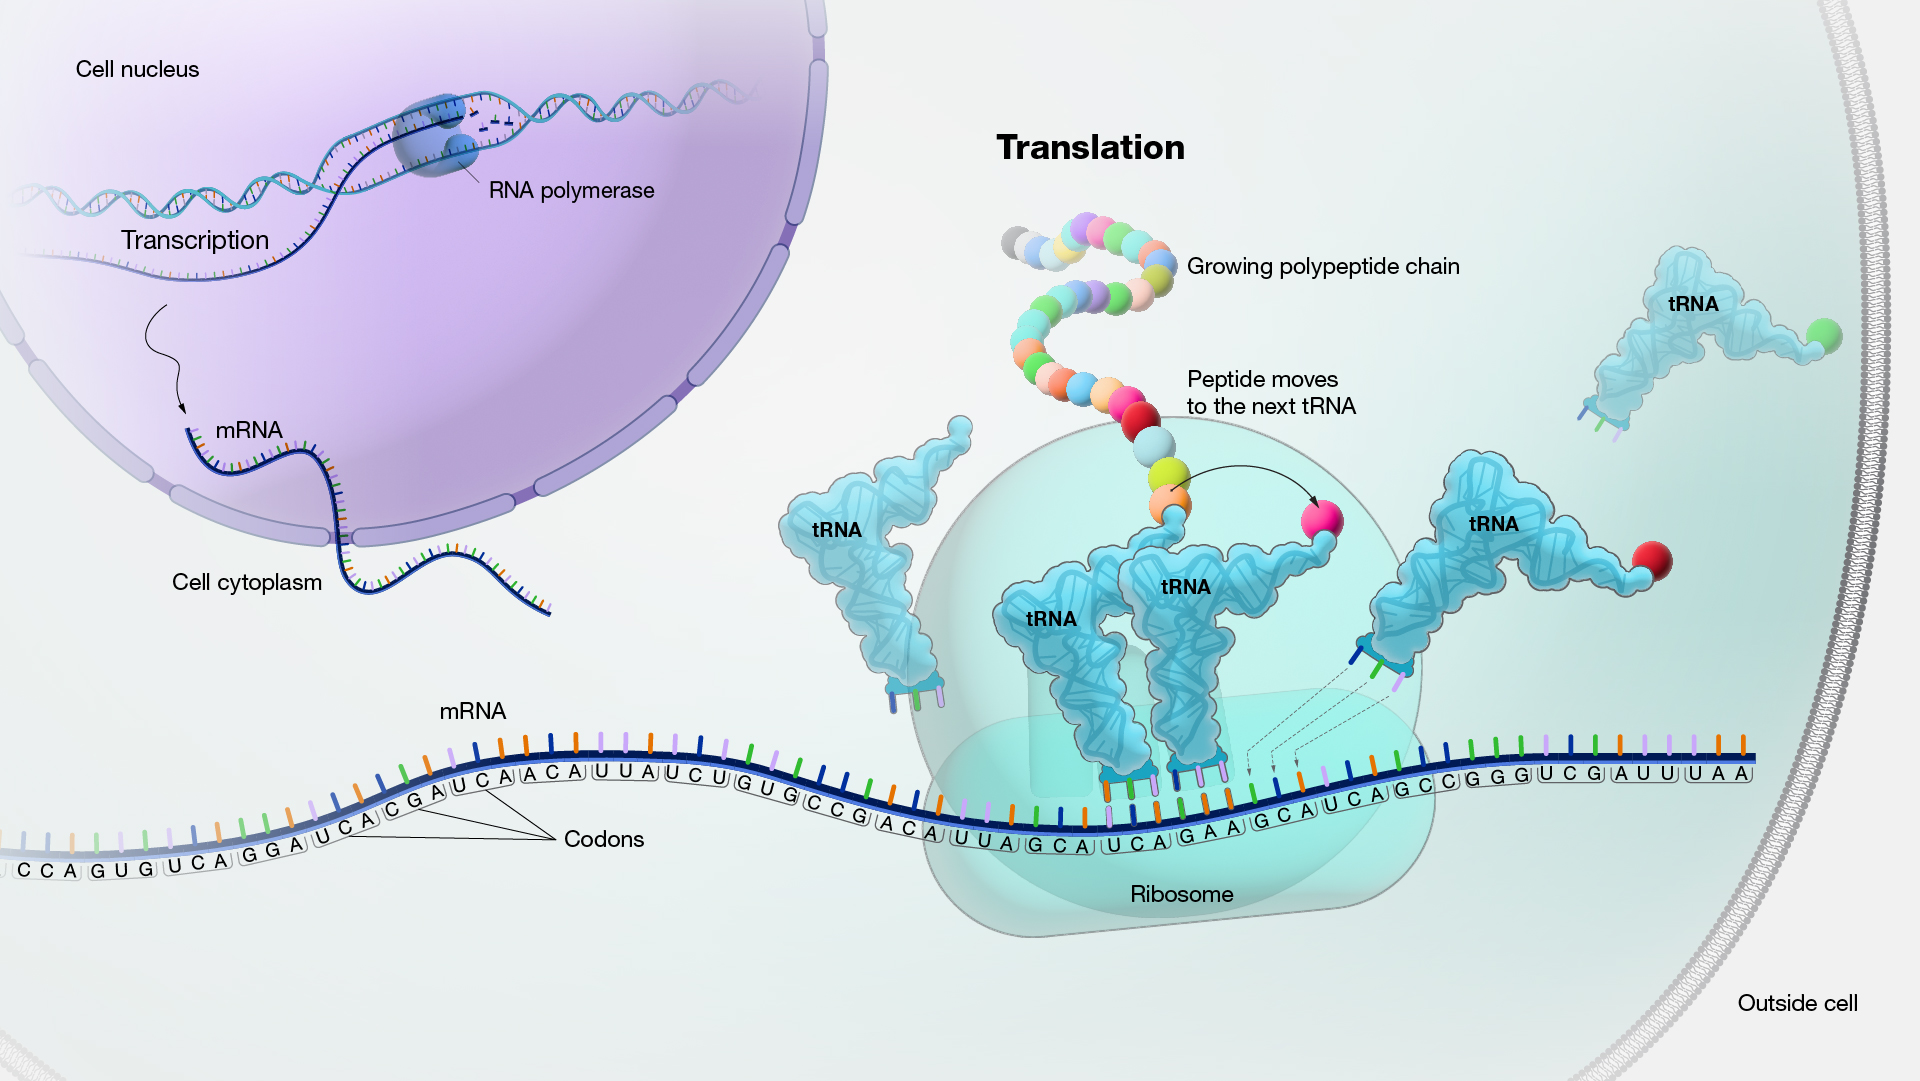
\includegraphics[width=\textwidth]{assets/mrna-translation.jpg}
    \caption[Il processo di traduzione da mRNA a polipeptide.]{Il processo di traduzione da RNA messaggero a polipeptide attraverso il tRNA e i ribosomi\,\cite{nhgri_translation_image}.}\label{fig:mrna-translation}
\end{figure}

Una volta creata la sequenza polipeptidica, inizia il processo di ripiegamento della proteina. In maniera molto simile a quanto visto per l'impacchettamento del DNA nel cromosoma, la sequenza di polipeptidi inizialmente si arrotola creando delle bobine che sono comunemente chiamate $\alpha$\textit{-helix}. Queste ultime poi si ripiegano nuovamente arrivando alla struttura terziaria della proteina, ovvero la proteina tridimensionale effettiva\,\cite{schulz2013principles}. Una volta creata la proteina il gene è stato espresso definitivamente. Questo passaggio di informazioni dal DNA alla creazione della proteina è gergo definito come il \textsl{dogma della biologia molecolare}.

Come accennato all'inizio del capitolo, la cellula possiede la notevole capacità di replicarsi. In genere una cellula si duplica durante la crescita e lo sviluppo dell'organismo, quando deve essere rimpiazzata o rigenerata oppure nella riproduzione asessuata di alcuni micro organismi\,\cite{bavle2014mitosis}. Il processo replicazione cellulare, chiamato \textsl{mitosi}, è preceduto dall'\textsl{interfase}, processo fondamentale in cui la cellula cresce di dimensioni e il DNA nei cromosomi si duplica, favorendo la replicazione cellulare. La mitosi può essere suddivisa in quattro fasi principali\,\cite{walczak2010mechanisms, bavle2014mitosis, li2020theoretical, sullivan2007finishing} le quali sono riassunte anche nella Figura\,\ref{fig:mitosis}:
\begin{enumerate}
    \item Nella \textsl{profase} i cromosomi duplicati si condensano nel nucleo ed iniziano ad avvicinarsi dei microtuboli al nucleo, chiamati \textsl{centrosomi}; allo stesso tempo la membrana nucleare inizia a svanire;
    \item Dopo che i microtuboli si sono attaccati ai cromosomi (fase intermedia detta \textsl{prometafase}) si giunge alla \textsl{metafase}, situazione in cui tutti i cromosomi sono allineati lungo la linea equatoriale della cellula;
    \item Durante l'\textsl{anafase}, ciascuna coppia di cromosomi si divide e raggiunge i poli della cellula;
    \item La fase finale della mitosi è la \textsl{telofase} nella quale le due cellule si dividono; le membrane nucleari delle due cellule si riformano attorno ai cromosomi divisi.
\end{enumerate}

\begin{figure}[b!]
    \centering
    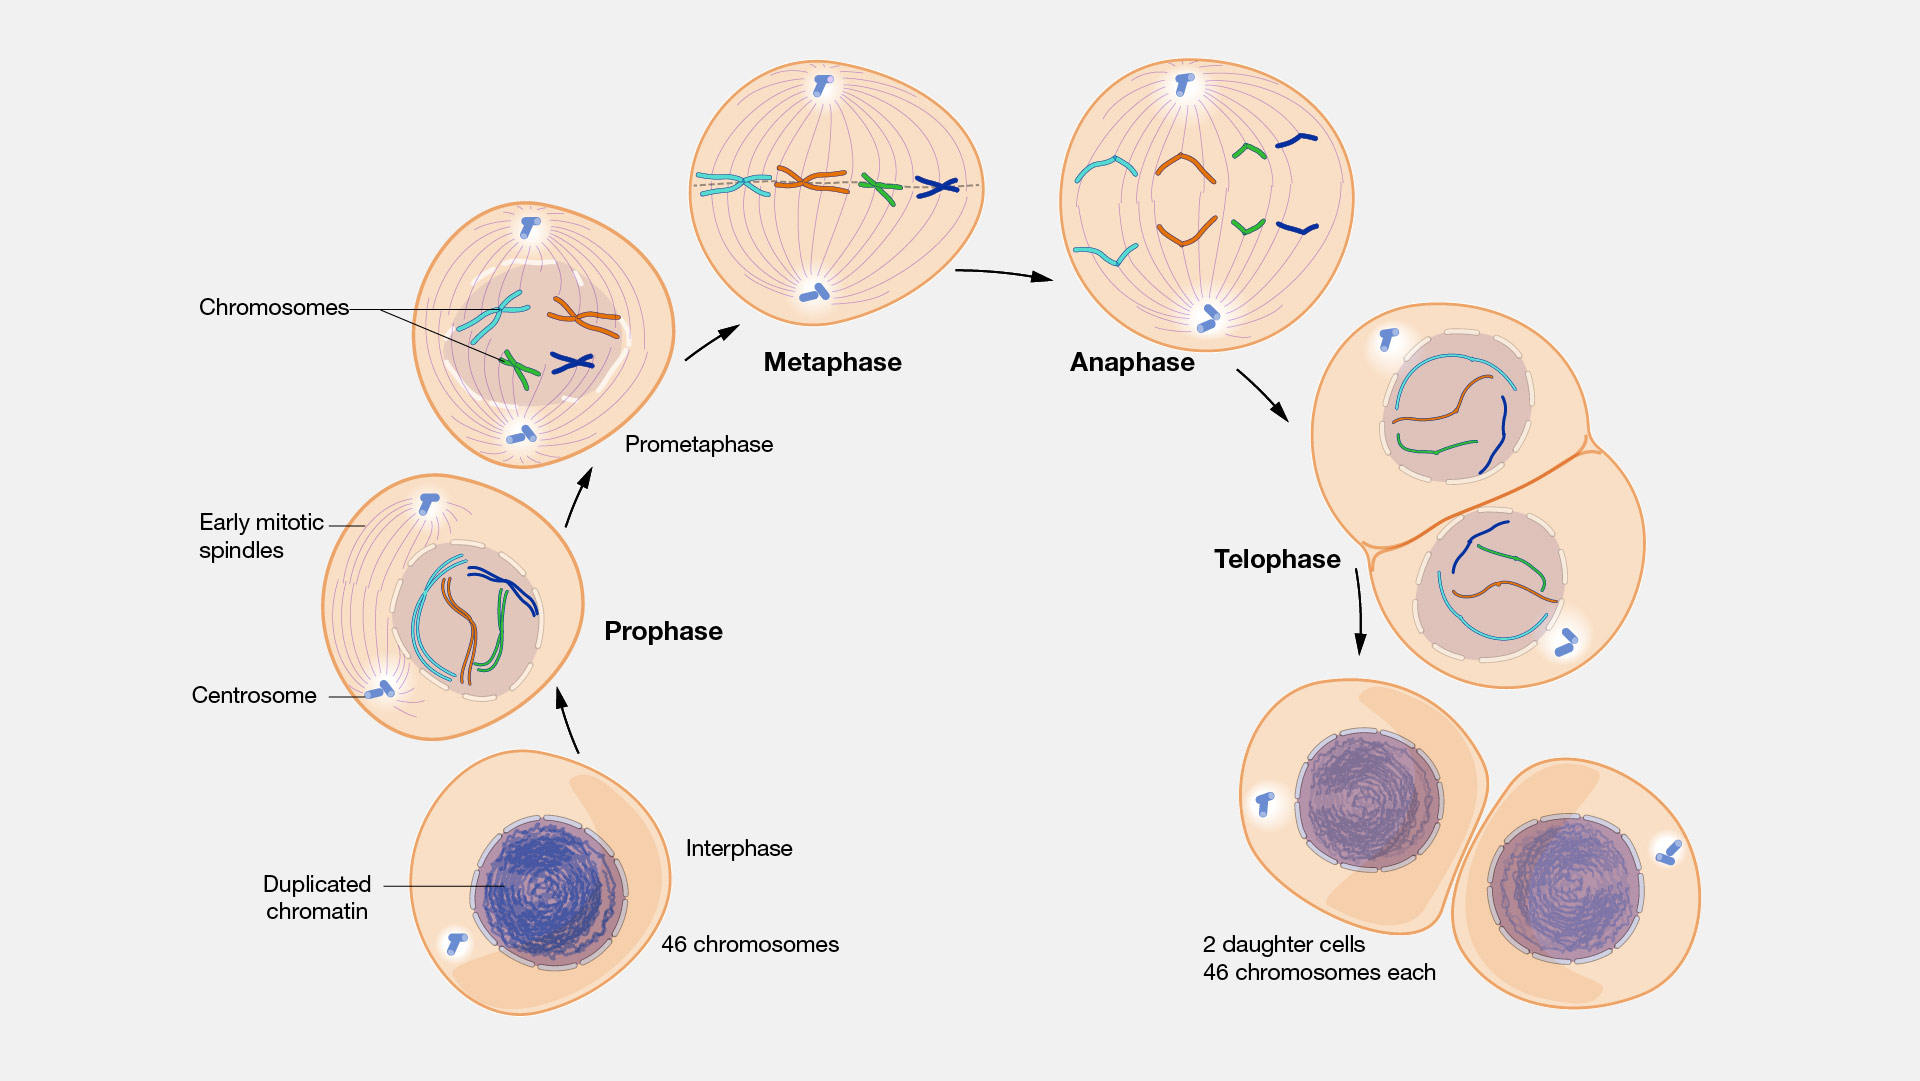
\includegraphics[width=\textwidth]{assets/mitosis.jpg}
    \caption[La mitosi cellulare.]{Rappresentazione delle quattro fasi che comprendono la mitosi cellulare\,\cite{nhgri_mitosis_image}.}\label{fig:mitosis}
\end{figure}

Affinché la mitosi abbia successo, è prima necessario duplicare il DNA all'interno della cellula. Il processo di replicazione di DNA che precede la mitosi è anche definito come \textsl{fase di sintesi} — \textit{S-phase}. La duplicazione del DNA inizia con l'identificazione dell'\textsl{origine della replicazione}, ovvero una sequenza del DNA che specifica da quale punto della sequenza il DNA deve essere replicato (ci sono più di cento mila siti che segnalano un punto di orine nel DNA di una cellula). Una \textsl{proteina iniziatrice} è legata al punto di origine promuovendo l'attaccamento al DNA del \textsl{replisoma} che è composto da un enzima chiamato \textsl{elicasi} che si occupa di dividere i due filamenti di DNA procedendo nella direzione $5^\prime \to 3^\prime$.\@ A questo punto il \textsl{RNA prime} inizia la sintesi del DNA favorendo l'attaccamento della \textsl{DNA polimerasi} entrambi i filamenti per duplicare il DNA.\@ Essendo che il genoma è complementare, un filamento avrà un verso $5^\prime \to 3^\prime$ (\textit{leading strand}) mentre l'altro filamento avrà verso opposto, $3^\prime \to 5^\prime$ (\textit{lagging strand}). Di conseguenza, nel filamento concorde al replisoma, la polimerasi non incontrerà problemi nella duplicazione, invece nel filamento $3^\prime \to 5^\prime$ il DNA dovrà essere duplicato a segmenti, detti \textsl{frammenti di Okazaki} che verranno collegati tramite la \textsl{DNA ligasi}\,\cite{laskey1989s, bell2002dna, dutta1997initiation, 2017727}. La Figura\,\ref{fig:dna-replication} racchiude quanto descritto sulla fase di sintesi.

\begin{figure}[b!]
    \centering
    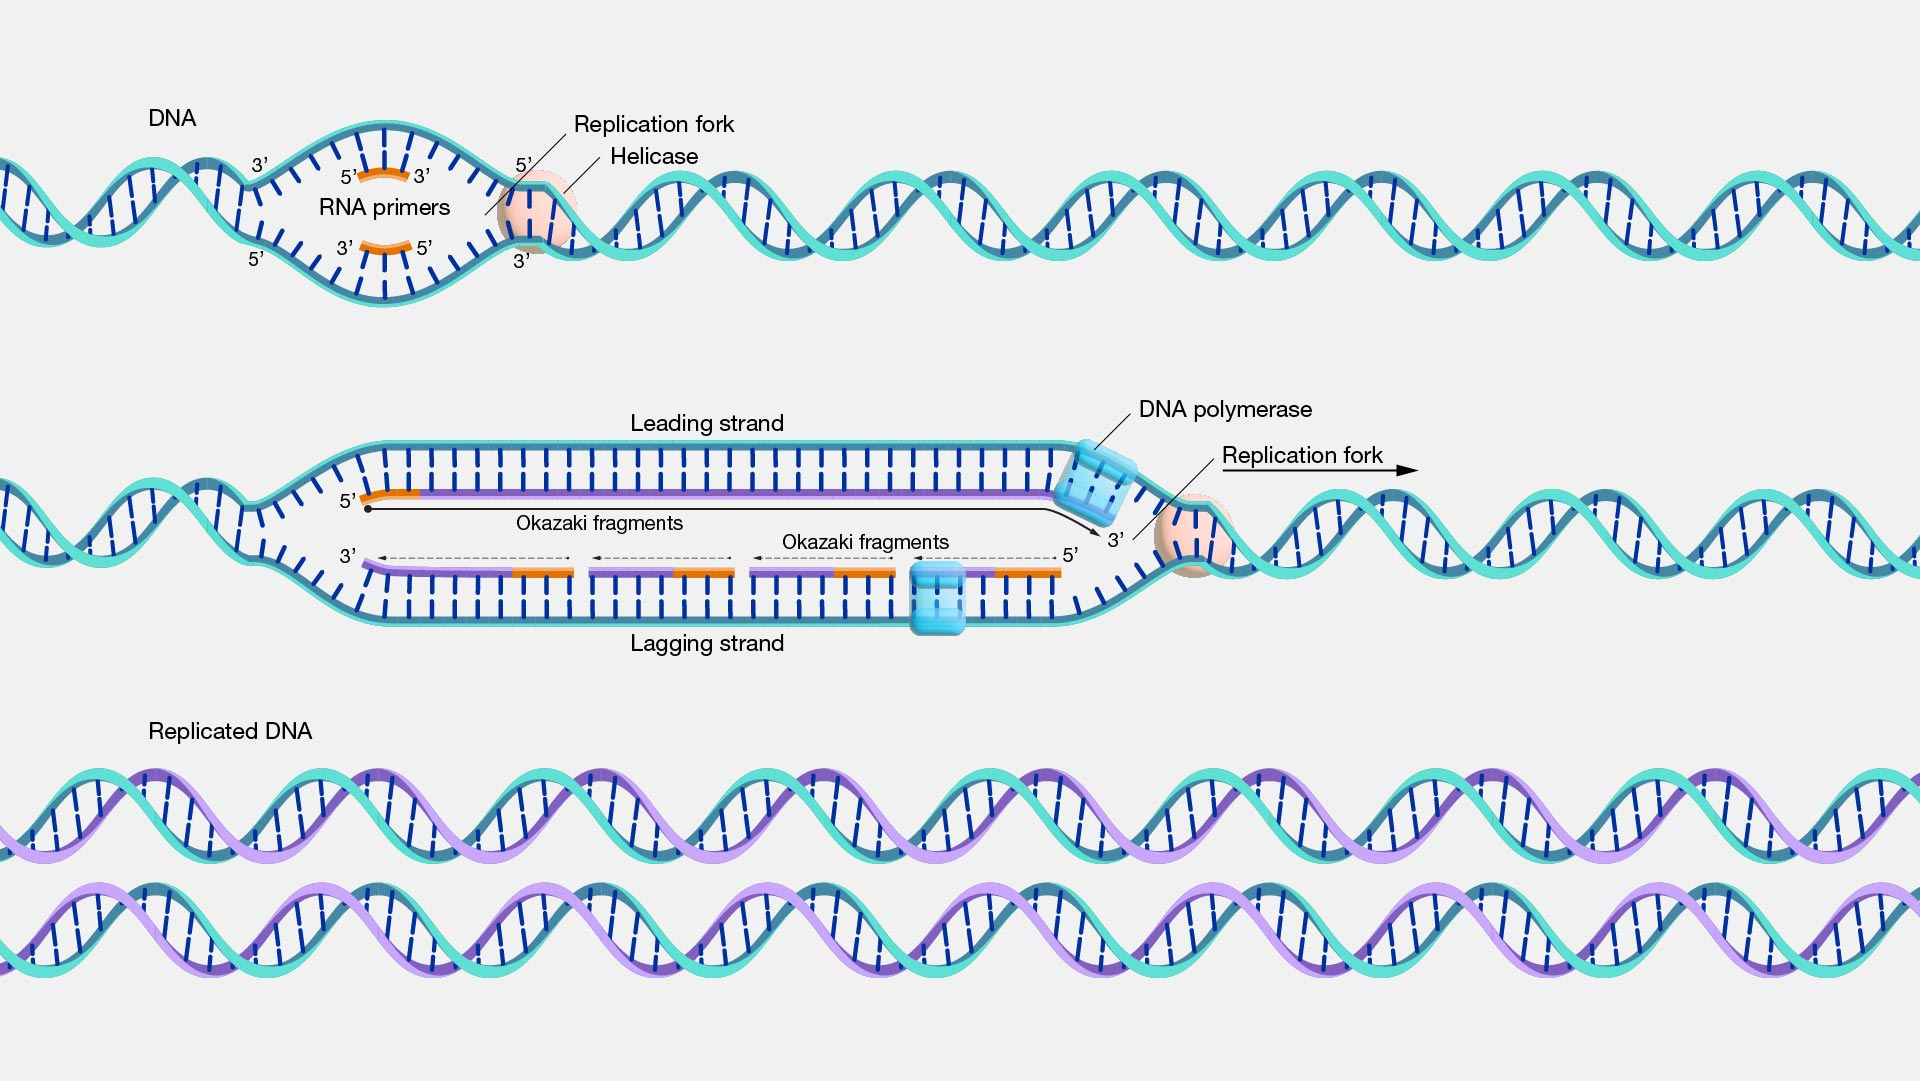
\includegraphics[width=\textwidth]{assets/dna-replication.jpg}
    \caption[Il processo di replicazione del DNA.]{Il processo di replicazione del DNA durante la fase di sintesi\,\cite{nhgri_dna_replication_image}.}\label{fig:dna-replication}
\end{figure}

\section{Varianti non codificanti}

Come descritto fino ad ora, il ruolo del DNA è fondamentale in quanto trasmesso da cellula a cellula durante la replicazione per poi essere utilizzato nell'espressione genica creando le proteine. Alle regioni del DNA che prendono parte al processo di espressione di un gene, si contrappongono le regioni che non vengono codificate, come le zone intensificatrici e promotrici del DNA e gli introni dei geni. Anche se queste sequenze non vengono effettivamente espresse, ricoprono un ruolo fondamentale nell'espressione genica (Figura\,\ref{fig:dna-transcription} e Figura\,\ref{fig:mrna-translation}) e durante la duplicazione del DNA (Figura\,\ref{fig:dna-replication}). Proprio per questo motivo le mutazioni in queste zone possono indurre a disturbi genetici critici. Ciò nonostante non si è ancora in grado di comprendere a fondo gli effetti che queste particolari mutazioni hanno. Risulta quindi importante continuare a studiare le varianti non codificanti e gli effetti collaterali genetici che provocano.


\todo{spiega in maniera più approfondita la varianti non codificianti}
    %!TEX root = ../main.tex

\chapter{Reti neurali}\label{chp:neural-networks}
% 
Il primo modello di intelligenza artificiale (\acs{AI}) risale al 1943, dove E. McCulloch e W. Pitts cercarono di modellare un neurone come una semplice funzione predefinita. Nel modello, il neurone, generava un valore in output nel caso in cui le variabili booleane di input, una volta elaborate, superavano una soglia prestabilita\,\cite[``A logical calculus of the ideas immanent in nervous activity'']{mcculloch1943logical}. Poco dopo, nel 1950, Alan Turing, pubblicò un articolo che definiva una metodologia per testare l'intelligenza di un modello\,\cite[``Computing machinery and intelligence'']{turing2009computing}. Questo test — noto anche come \textit{imitation game} — consisteva nel valutare se una macchina potesse imitare l'intelligenza umana tabilendo così un obiettivo per il campo dell'intelligenza artificiale, termine che venne conianto per la prima volta nella conferenza di Dartmouth nel 1956.

Dopo due anni, nel 1958, lo psicologo F. Resenblatt introdusse il \textsl{percettrone} che, a differenza del modello del '43, processava input non booleani e disponeva di pesi per bilanciare l'output\,\cite[``The perceptron: a probabilistic model for information storage and organization in the brain.'']{rosenblatt1958perceptron}. Anche se il percettrone sarà alla base delle reti neurali artificiali moderne, nei dieci anni successivi alla pubblicazione dell'articolo, le aspettative iniziali non vennero soddisfatte. Nel 1968 venne pubblicato un libro il quale analizzava le prestazioni del percettrone e constatava le forti limitazioni del modello, come l'impossibilità di risolvere problemi non linearmente separabili\,\cite[``Perceptrons'']{minsky2017perceptrons}. In seguito ad un secondo articolo del 1973, dove si evidenziavano gli scarsi risultati ottenuti in paragone con le grandi aspettative, iniziò il \textsl{Primo Inverno dell'Intelligenza Artificiale} dove fino alla metà degli anni Ottanta molte organizzazioni governative smisero di finanziare la ricerca sull'Intelligenza Artificiale (\acs{AI}). L'Inverno della \acs{AI} terminò nel 1985 con l'introduzione del \textit{Gradient Descent Optimization}, algoritmo che permetteva di aggiornare i pesi in modo tale da minimizzare l'errore in una rete. Un anno dopo venne introdotto l'algoritmo della \textit{back-propagation}, fondamentale per lo sviluppo di reti neurali, costituite da più livelli di neuroni, ciascuno dei quali è collegato al livello successivo\,\cite[``Learning representations by back-propagating errors'']{rumelhart1986learning}.

Nonostante il grande sviluppo nella parte algoritmistica, l'hardware non era computazionalmente prestante da supportare le richieste di calcolo delle reti neurali artificiali. Questa carenza nella potenza di calcolo portò al \textsl{Secondo Inverno dell'Intelligenza Artificiale}, periodo in cui l'interesse scientifico si spostò su modelli che richiedevano meno potenza di calcolo, come le \textit{Support Vector Machines} (\acs{SVM}) introdotte nel 1963. Il Secondo Inverno della \acs{AI} terminò a metà degli anni Novanta quando il progresso dell'hardware riuscì a soddisfare i requisiti computazionali dei modelli basati su reti neurali. Il costante sviluppo culminò nell'ultimo ventennio quando venne introdotta la \acs{GPU}, che, insieme all'aumento dei dati disponibili, accelerò notevolmente i progressi nel campo dell'\acs{AI}\,\cite{flasinski2016introduction, muthukrishnan2020brief}.

\section{Principi di base ed evoluzione}
%
Le reti neurali artificiali (\acs{ANN}) — comunemente note come reti neurali (\acs{NN}) — mirano a rappresentare un modello semplificato del cervello, trattato come una struttura composta da neuroni. Risulta quindi essenziale comprendere il funzionamento del singolo \textsl{neurone artificiale} per poi esplorare la struttura di una rete neurale, che è un collegamento tra più neuroni artificiali.

Come un neurone biologico, il neurone artificiale (Figura\,\ref{fig:artificial-neuron}) riceve un numero indefinito $n$ di segnali in \textsl{input}, che possono essere rappresentati con la notazione $x_0, x_1, \dots, x_n$. Tali valori possono essere raggruppato nel vettore di input $\mathbf{x} = \left[x_0, x_1, \dots, x_n\right]$. Per descrivere il risultato di tutti i segnali in ingresso del neurone, si introduce una funzione $g$, che generalmente è una semplice somma algebrica dei segnali di input $x_i$, con $i\in[0,\,n]$. Ogni segnale di input, prima di essere sommato viene moltiplicato per il rispettivo peso (\textit{weight}) $w_i$, con $i\in[0,\,n]$, che appartiene al vettore dei pesi $\mathbf{w} = \left[w_0, w_1, \dots, w_n \right]$. Ne consegue che il segnale in uscita, indicato con $v$, comprenderà la somma del prodotto del segnale \textit{i}-esimo ($x_i$) con il rispettivo peso \textit{i}-esimo ($w_i$):
% 
\begin{gather}
    v = g\left(\mathbf{w}, \mathbf{x}\right) = \sum_{i = 0}^n w_i\,x_i = \mathbf{w}\,\cdot\,\mathbf{x}
    \label{eq:algebric-sum}
\end{gather}
% 
\begin{figure}[!b]
    \centering
    \begin{tikzpicture}[node distance=1cm, auto]

    % inputs
    \node[draw, rectangle] (X0) {$x_0$};
    \node[below of=X0] (dots1) {$\vdots$};
    \node[draw, rectangle, below of=dots1] (Xi) {$x_i$};
    \node[below of=Xi] (dots2) {$\vdots$};
    \node[draw, rectangle, below of=dots2] (Xn) {$x_n$};
    
    % perceptron summation
    \node [draw, circle, right=2.5cm of Xi, minimum size=1.5cm] (perceptron) {\large $\displaystyle \sum$};

    % signal output v
    \node [right=0.5cm of perceptron] (output) {};

    % activation function f(v)
    \node [draw, rectangle, right=0.5cm of output] (activation) {$f(v)$};

    % final output y
    \node [right=1cm of activation] (final_output) {};

    % input arrows with weights
    \draw [->] (X0) -- node[midway, above] {} node[midway,below] {$w_0$} (perceptron);
    \draw [->] (Xi) -- node[midway, above] {} node[midway,below] {$w_i$} (perceptron);
    \draw [->] (Xn) -- node[midway, above] {} node[midway,below] {$w_n$} (perceptron);

    \draw [->] (perceptron) -- node[above] {$v$} (activation);

    \draw [->] (activation) -- node[above] {$y$} (final_output);

\end{tikzpicture}
    \caption[Rappresentazione schematica del funzionamento di un neurone artificiale.]{Rappresentazione schematica del funzionamento di un neurone artificiale. I segnali in input $X_i$ vengono moltiplicati con i rispettivi pesi $W_i$ e sommati tra loro; il risultato $v$ viene processato dalla funzione di $f(v)$ che restituisce l'output $z$.}\label{fig:artificial-neuron}
\end{figure}
% 
\noindent Per attivare un neurone, è necessario che il segnale $v$ prodotto in \textsl{output} sia superiore ad una soglia prescelta, solitamente rappresenta dalla prima componente del vettore di input ($x_0$). Questo valore, noto come \textit{bias}, è scelto arbitrariamente ma spesso viene impostato ad 1. Il criterio che descrive l'attivazione del neurone artificiale è riassunto nella \textsl{funzione di attivazione}, chiamata $z = f(v)$. La funzione di attivazione più semplice che descrive tale criterio la funzione \textsl{gradino} \textbf{1}$(v)$, descritta graficamente nella Figura\,\ref{fig:step-function}:
% 
\begin{gather*}
    z(v) = \text{\textbf{1}}(v) =
    \begin{cases}
        1 \hspace{20px} \text{se } v\geq0\\
        0 \hspace{20px} \text{se } v<0
    \end{cases}
\end{gather*}
% 
\begin{figure}[!b]
    \centering
    \begin{tikzpicture}
    \begin{axis}[
        axis lines = middle,
        xlabel = $v$,
        ylabel = {\textbf{1}$(v)$},
        ymin=-0.2, ymax=1.2, % control the vertical limits
        xmin=-3, xmax=3,     % control the horizontal limits
        xtick={-2,-1,0,1,2}, % x-axis ticks
        ytick={0,1},         % y-axis ticks
        domain=-3:3,
        samples=100,
        width=10cm,
        height=6cm,
        enlargelimits
    ]
        % Plot the step function
        \addplot[
            red,
            thick,
            domain=-3:0,
        ] {0}; % Plot f(x) = 0 for x < 0

        \addplot[
            red,
            thick,
            domain=0:3,
        ] {1}; % Plot f(x) = 1 for x >= 0

        % Add a filled circle for the closed part of the step at x = 0, y = 1
        \addplot[only marks, mark=*, black] coordinates {(0, 1)};
        
        % Add an open circle for the open part of the step at x = 0, y = 0
        \addplot[only marks, mark=o, black] coordinates {(0, 0)};
        
    \end{axis}
\end{tikzpicture}
    \caption[Grafico della funzione gradino \textsl{1}$(v)$.]{Grafico della funzione gradino \textbf{1}$(v)$. Si osserva che vale zero per valori strettamente minori di zero e uno per valori maggiori o ugali a zero.}\label{fig:step-function}
\end{figure}
% 
\noindent Come per un cervello umano, anche la rete neurale deve essere in grado di impararare. In particolare un neurone artificiale deve essere in grado di reagire in un determinato modo quando in input riceve determinati \textsl{pattern}. Affinchè il neurone sia in grado di comporatarsi correttamente di fronte a dei pattern, è fondamentale allenarlo: è dunque necessario utilizzare un \textit{training dataset} che contenga numerosi vettori di input $\mathbf{x}$ e, per ciascuno di essi sia presente la risposta corretta che il neurone dovrebbe fornire. Formalmente definiamo il dataset $\mathcal{D}$ come:
% 
\begin{gather*}
    \mathcal{D} = \left\{ \left\{ X_1,\, y_1 \right\},\,\left\{ X_2,\, y_2 \right\},\,\dots\,\left\{ X_j,\, y_j \right\},\,\dots\,\left\{ X_M,\, y_M \right\} \right\}  
\end{gather*}
% 
\noindent Il dataset\footnote{Un dataset così definito è utilizzato nel \textit{supervised learning}, dove all'interno del dataset sono presenti sia i vettori in ingresso che la risposta attesa. Si contrappone l'\textit{unsupervised learning} — che non verrà trattato — dove sono presenti solo i vettori in ingresso e sono sconosciute le risposte attese.} è composto da $M$ vettori di input, definiti con la notazione $X_j$ ($j\in[1,\,M$]), e da esattamente $M$ risposte $y_j$, che rappresentano il comportamento atteso del neurone se il vettore di ingresso è $X_j$. È quindi possibile definire la matrice $\mathbf{X}$ che contiene esattamente $M$ vettori — ciascuno in una riga — i quali sono composti esattamente da $n$ componenti (o \textit{feature}), che sono le componenti associate al vettore dei pesi $\mathbf{w}$, precedentemente introdotto. Alla matrice $\mathbf{X}$ è associato il vettore $\mathbf{y}$, anch'esso di dimensione $M$ tale per cui la componente $y_j$ sia la risposta attesa del vettore di input $X_j$.
% 
\begin{gather*}
    \begin{aligned}
        \mathbf{X} &= 
            \begin{bmatrix}
            X_1^0       & X_1^1         & \cdots     & X_1^i         & \cdots     & X_1^n     \\
            X_2^0       & X_2^1         & \cdots     & X_2^i         & \cdots     & X_2^n     \\
            \vdots      & \vdots        & \ddots     & \vdots        & \ddots     & \vdots    \\
            X_j^0       & X_j^1         & \cdots     & X_j^i         & \cdots     & X_j^n     \\
            \vdots      & \vdots        & \ddots     & \vdots        & \ddots     & \vdots    \\
            % X_{M-1}^0   & X_{M-1}^1     & \cdots     & X_{M-1}^i     & \cdots     & X_{M-1}^n \\
            X_M^0       & X_M^1         & \cdots     & X_M^i         & \cdots     & X_M^n     \\
            \end{bmatrix}
        %
        \hspace{60px}
        %
        \mathbf{y} = 
            \begin{bmatrix}
            y_1 \\ y_2 \\ \vdots \\ y_j \\ \vdots \\ y_M
            \end{bmatrix}
    \end{aligned}
\end{gather*}
% 
\noindent Da questo deriva che il vettore $X_j$ è dimensionalmente compatibile con il vettore di pesi $\mathbf{w}$ in quanto hanno esattamente la stessa dimensione.
% 
\begin{gather*}
    \begin{aligned}
        X_j = \left[ X_j^0,\, X_j^1,\,\dots,\, X_j^n \right]
        %
        \hspace{50px}
        %
        \mathbf{w} = \left[w_0,\, w_1,\, \dots,\, w_n \right]
    \end{aligned}
\end{gather*}
% 
\noindent Perciò il dataset $\mathcal{D}$ può essere riscritto attraverso la matrice $\mathbf{X}$ ed il vettore di risposte attese associato $\mathbf{y}$.
% 
\begin{gather*}
    \mathcal{D} = \left\{ \mathbf{X},\, \mathbf{y} \right\}  
\end{gather*}
% 
Con un dataset di partenza si può definire un algoritmo generico che sia in grado di descrivere il processo di apprendimento di neurone artificiale. Come descritto nell'Algoritmo\,\ref{alg:neuron-training}, dopo aver inizializzato il vettore di pesi $\mathbf{w}$, per ogni vettore $X_j$ del dataset $\mathcal{D}$ vengono calcolati il segnale $v$ e il valore della funzione di attivazione $z = f(v)$. L'idea alla base dell'algoritmo è quella di modificare il vettore di pesi $\mathbf{w}$ in funzione del risultato della funzione di attivazione rispetto al segnale processato.
% 
\begin{algorithm}[ht]
    \caption{Allenamento del neurone artificiale}\label{alg:neuron-training}
    \begin{algorithmic}
        \STATE{\textbf{Input: }Dataset $\mathcal{D}$}
        \STATE

        \STATE{Inizializza $\mathbf{w}$ con numeri casuali}
        \STATE$j \gets 1$
        
        \WHILE{$j \leq M$}
            \STATE\text{Calcola $v$ in funzione di $X_j$ e $\mathbf{w}$}
            \STATE\text{Determina $z$ in rapporto a $v$ e $y_j$}
            \STATE\text{Modifica $\mathbf{w}$ a seconda del risultato $z$}
            \STATE$j \gets j + 1$
        \ENDWHILE\,
    \end{algorithmic}
\end{algorithm}
% 
\noindent In questo modo, una volta processati tutti i vettori presenti nel dataset, è possibile constatare se il neurone sia stato in grado di apprendere il comportamento desiderato in funzione del vettore in ingresso\,\cite{flasinski2016introduction}.

Uno tra i modelli di neuroni artificiali utilizzati nelle reti neurali è il percettrone. Dato un vettore in ingresso $X_j$ e un vettore di pesi $\mathbf{w}$, il segnale $v$ è dato dalla somma algebrica dei prodotti di ciascuna delle componenti:
% 
\begin{gather*}
    v = g\left(\mathbf{w}, X_j\right) = \sum_{i = 0}^n w_i\,X_j^i = \mathbf{w} \, \cdot \,  X_j
\end{gather*}
% 
\noindent La funzione di attivazione $f(v)$ del percettrone è la funzione \textsl{``segno''}\,(Figura\,\ref{fig:sign-function}), chiamata anche \textsl{gradino bipolare} e definita come segue. 
% 
\begin{figure}[!t]
    \centering
    \begin{tikzpicture}
    \begin{axis}[
        axis lines = middle,
        xlabel = $v$,
        ylabel = {\textbf{sign}$(v)$},
        ymin=-1.2, ymax=1.2, % control the vertical limits
        xmin=-3, xmax=3,     % control the horizontal limits
        xtick={-2,-1,0,1,2}, % x-axis ticks
        ytick={-1,0,1},      % y-axis ticks
        domain=-3:3,
        samples=100,
        width=10cm,
        height=6cm,
        enlargelimits,
        yticklabel style={yshift=-1ex, xshift=0.75ex} % Adjust vertical position of y-tick labels
    ]
        % Plot the step function
        \addplot[
            red,
            thick,
            domain=-3:0,
        ] {-1}; % Plot f(x) = -1 for x < 0

        \addplot[
            red,
            thick,
            domain=0:3,
        ] {1}; % Plot f(x) = 1 for x >= 0

        % Add a filled circle for the closed part of the step at x = 0, y = 1
        \addplot[only marks, mark=*, black] coordinates {(0, 1)};
        
        % Add an open circle for the open part of the step at x = 0, y = 0
        \addplot[only marks, mark=o, black] coordinates {(0, -1)};
        
    \end{axis}
\end{tikzpicture}

    \caption[Grafico della funzione segno \textsl{sign}$(v)$.]{Grafico della funzione segno \textbf{sign}$(v)$. Si osserva che vale -1 per valori strettamente minori di zero e 1 per valori maggiori o ugali a zero.}\label{fig:sign-function}
\end{figure}
% 
\begin{gather*}
    z(v) = \text{\textbf{sign}}(v) = \text{\textbf{sign}}(\mathbf{w} \cdot X_j) =
    \begin{cases}
        1 \hspace{29px} \text{se } v\geq0\\
        -1 \hspace{20px} \text{se } v<0
    \end{cases}
\end{gather*}
% 
\noindent Il particolare più importante del percettrone però è la \textit{learning rule}, ovvero il criterio secondo il quel il vettore di pesi è aggiornato a seconda della predizione del modello. Se la predizione $z_j$ rispetto al vettore $X_j$ è diversa dalla risposta attesa $y_j$, allora il vettore di pesi è modificato come segue\,\cite{nielsen2015neural, flasinski2016introduction}.
% 
\begin{gather*}
    w_i \, = \, w_i \, + \, y_j\,X_j^i
\end{gather*}

Al percettrone si aggiunge anche il \textsl{neurone sigmoideo}, che è molto simile al percettrone se non per la funzione di attivazione. Anzichè avere la funzione discontinua ``segno'', viene introdotta la funzione \textsl{sigmoide} $\sigma(v)$, che è una funzione continua e restituisce valori compresi tra zero e uno (Figura\,\ref{fig:sigmoid-function}). Questa funzione, definita di seguito, rimuove le discontinuità della funzione di attivazione del percettrone e fornisce un raggio di valori reali, piuttosto che un risultato booleano.
% 
\begin{gather*}
    \sigma(v) \, = \, \frac{1}{1 + e^{-v}} \, = \, \frac{1}{1 + e^{-\mathbf{w} \cdot X_j}}
\end{gather*}
% 
\begin{figure}[!t]
    \centering
    \begin{tikzpicture}
    \begin{axis}[
        axis lines = middle,
        xlabel = $v$,
        ylabel = {$\sigma(v)$},
        ymin=-0.1, ymax=1.1, % control the vertical limits
        xmin=-5, xmax=5,     % control the horizontal limits
        xtick={-4,-2,0,2,4}, % x-axis ticks
        ytick={0,0.5,1},     % y-axis ticks
        domain=-5:5,
        samples=100,
        width=10cm,
        height=6cm,
        enlargelimits,
        yticklabel style={yshift=-1ex, xshift=0.75ex} % Adjust vertical position of y-tick labels
    ]
        % Plot the sigmoid function
        \addplot[
            red,
            thick
        ] {1 / (1 + exp(-x))};
        
        % Add horizontal lines at y = 1 for reference
        \addplot[dashed] coordinates {(-5,1) (5,1)} node[right] {};
    \end{axis}
\end{tikzpicture}

    \caption[Grafico della funzione sigmoide $\sigma(v)$.]{Grafico della funzione sigmoide $\sigma(v)$.}\label{fig:sigmoid-function}
\end{figure}
% 
Questa importante differenza rende il neurone sigmoideo più flessibile rispetto al percettrone classico e più adatto all'utilizzo nelle reti neurali\,\cite{nielsen2015neural}.

La learning rule introdotta nel percettrone, per quanto semplice, spesso viene sostituita dalla learning rule derivante dal \textit{Gradient Descent} (\acs{GD}), un approccio che mira a trovare il minimo di una funzione differenziabile, spesso chiamata funzione ``costo''. Fornito il vettore di pesi $\mathbf{w} = \left[w_0, w_1, \dots, w_n \right]$, durante l'allenamento del neurone, l'algoritmo cerca di modificare tale vettore cercando di minimizzare sempre di più l'errore tra il valore predetto dal modello e il risultato atteso. Più precisamente, data una funzione di costo $C(w)$ — detta anche \textit{loss function} — la learning rule del \acs{GD} vale:
% 
\begin{gather*}
    \mathbf{w} = \mathbf{w} - \eta\,\nabla C\left(\mathbf{w}\right)
\end{gather*}
% 
\begin{figure}[!b]
    \centering
    \tikzset{arrowed/.style={
    decorate,
    decoration={
        show path construction, 
        moveto code={},
        lineto code={
            \draw[#1] (\tikzinputsegmentfirst) -- (\tikzinputsegmentlast);
        },
        curveto code={},
        closepath code={},
    }
}, arrowed/.default={-stealth}}

\pgfplotsset{
    gradient function/.initial=f,
    dx/.initial=0.01,
    dy/.initial=0.01
}

\pgfmathdeclarefunction{xgrad}{2}{%
    \begingroup%
    \pgfkeys{/pgf/fpu,/pgf/fpu/output format=fixed}%
    \edef\myfun{\pgfkeysvalueof{/pgfplots/gradient function}}%
    \pgfmathparse{(\myfun(#1+\pgfkeysvalueof{/pgfplots/dx},#2)%
        -\myfun(#1,#2))/\pgfkeysvalueof{/pgfplots/dx}}%
    \pgfmathsmuggle\pgfmathresult%
    \endgroup%
}

\pgfmathdeclarefunction{ygrad}{2}{%
    \begingroup%
    \pgfkeys{/pgf/fpu,/pgf/fpu/output format=fixed}%
    \edef\myfun{\pgfkeysvalueof{/pgfplots/gradient function}}%
    \pgfmathparse{(\myfun(#1,#2+\pgfkeysvalueof{/pgfplots/dy})%
        -\myfun(#1,#2))/\pgfkeysvalueof{/pgfplots/dy}}%
    \pgfmathsmuggle\pgfmathresult%
    \endgroup%
}

\pgfplotsset{compat=1.17}

\begin{tikzpicture}
    \begin{axis}[width=12cm,
        declare function={
            f(\x,\y)=cos(deg(\x)*0.8)*cos(deg(\y)*0.7)*exp(0.3*\x);
        },
        colormap/cool % Change the colormap here
    ]
        \addplot3[
            surf,
            shader=interp,
            domain=-4:3
        ]{f(x,y)};
        
        \edef\myx{1} % First x coordinate
        \edef\myy{0.25} % First y coordinate
        \edef\mystep{-0.25} % Negative values mean descending
        \pgfmathsetmacro{\myf}{f(\myx,\myy)}
        \edef\lstCoords{(\myx,\myy,\myf)}
        
        \pgfplotsforeachungrouped\X in{0,...,5}
        {
            \pgfmathsetmacro{\mydx}{xgrad(\myx,\myy)}
            \pgfmathsetmacro{\mydy}{ygrad(\myx,\myy)}
            \pgfmathsetmacro{\myscale}{\mystep/sqrt(\mydx*\mydx+\mydy*\mydy)}
            \pgfmathsetmacro{\myx}{\myx+\myscale*\mydx}
            \pgfmathsetmacro{\myy}{\myy+\myscale*\mydy}
            \pgfmathsetmacro{\myf}{f(\myx,\myy)}
            \edef\lstCoords{\lstCoords\space (\myx,\myy,\myf)}
        }
        
        \addplot3[
            samples y=0,
            arrowed,
            yellow,
            thick
        ] coordinates \lstCoords;
    \end{axis}
\end{tikzpicture}
    \caption[Funzionamento del gradient descent in una funzione bidimensionale.]{Funzionamento del gradient descent in una funzione bidimensionale. Si osserva che l'algoritmo, attraverso il gradiente della funzione, riesce a spostarsi verso il minimo (locale o assoluto) della funzione, come una biglia di vetro.}\label{fig:gradient-descent}
\end{figure}
% 
\noindent Dove $\eta$ è un parametro positivo, chiamato \textit{learning rate} e serve per bilanciare la rapidità con cui il vettore dei pesi sia aggiornato durante l'esecuzione dell'algoritmo. Il termine $\nabla C\left(\mathbf{w}\right)$ è invece il gradiente della loss function. Il gradiente di una funzione a più dimensioni è un vettore la cui direzione fa aumentare più rapidamente il valore della funzione; conseguentemente la direzione opposta è la direzione da seguire per raggiungere il minimo della funzione. La Figura\,\ref{fig:gradient-descent} mostra graficamente come l'approccio \acs{GD} cerchi di raggiungere il minimo della funzione costo ad ogni iterazione. Si osserva che in questo caso la funzione costo è rappresentata in due dimensioni ma in genera questa è una funzione $n$-dimensionale. Questa funzione può essere una qualsiasi funzione errore: una tra le più comuni è la funzione che calcola la media del quadrato degli errori (in gergo chiamata \acs{MSE}, \textit{Mean Squared Errors}). Per fare un esempio pratico, avendo il vettore di pesi $\mathbf{w}$, un dataset $\mathcal{D}$ — definito come in precedenza — ed una funzione di attivazione $z$, la \acs{MSE} è definita come:
% 
\begin{gather*}
    C(\mathbf{w}) = \frac{1}{M}\,\sum_{j = 1}^M\,{\left[ y_j - z(\mathbf{w},\,X_j) \right]}^2
\end{gather*}
% 
\noindent L'approccio adottato da questo algoritmo, per quanto efficacie non è completamente efficiente. La complessità computazionale richiesta è notevole: ad ogni iterazione dell'allentamento del neurone, è necessario travare il valore della derivata della loss function, che si traduce nel computare la predizione di tutti i vettori di input $X_j$ del dataset $\mathcal{D}$ e compararli con la risposta attesa $y_j$. Questo approccio, per dataset di dimensioni medio-grandi è molto poco efficiente, per quanto preciso. Inoltre è possibile che la discesa del gradiente conduca l'aggiornamento del vettore di pesi in un minimo locale della funzione errore, giungendo quindi ad una soluzione sub-ottima. Questi probliemi possono entrambi essere gestiti da una variante di questo algoritmo, chiamata \textit{Stochastic Gradient Descent} (\acs{SGD}). Per ogni iterazione dell'algoritmo di allenamento, vengono presi un numero $m < M$ di vettori di input con le rispettive risposte attese e aggiornato il vettore $\mathbf{w}$ in base a questo sotto insieme del dataset, chiamato anche $mini-batch$. In questo modo la complessità computazionale viene drasticamente diminuita in quanto calcolare la derivata della loss function per una frazione ridatta del dataset richiede meno risorse. In aggiunta la casualità della scelta del mini-batch può evitare la convergenza in un minimo locale poichè rende la discesa lungo la funzione di errore leggermente più imprevedibile, diminuendo la possibilità di risultati sub-ottimi. Questo approccio è così importante ed efficace che viene ad oggi utilizzato per allenare le reti neurali\,\cite{lu2022gradient, andrychowicz2016learning, nielsen2015neural}.

Una rete neurale è una struttura composta da neuroni artificiali i quali sono organizzati in livelli (\textit{layers}). In una rete neurale multilivello, è sempre presente un input layer e un output layer. I livelli che si trovano tra questi sono detti livelli nascosti — \textit{hidden} layers. Va osservato che i neuroni dello stesso livello non sono mai collegati ma sono collegati con quelli del livello precedente e del livello successivo.
% 
\begin{figure}[!b]
    \centering
    % see this link
% https://tikz.net/neural_networks/

    \caption[Rappresentazione di una rete neurale multilivello.]{Rappresentazione di una rete neurale multilivello.}\label{fig:neural-network}
\end{figure}
% 
In particolare, data una rete neurale, i neuroni del livello $\ell$ ricevono il segnale dai neuroni del livello $\ell-1$ e, dopo aver elaborato le informazioni, inviano il segnale processato i neuroni del livello $\ell+1$: si dice che la rete è di tipo \textit{feedforward} in quanto non sono presenti cicli nella struttura. Osservando la Figura\,\ref{fig:neural-network} si introduce una nuova notazione per le reti neurali: si definisce con $N^{(\ell)}_j$ il neurone $j$-esimo che si trova nel livello $\ell$; conseguentemente l'output della sua funzione di attivazione è identificato da $a^{(\ell)}_j$. Il peso $w^{(\ell)}_{j\,,i}$ è il peso che collega il neurone $N^{(\ell - 1)}_i$ al neurone $N^{(\ell)}_j$, ovvero il collegamento tra il neurone alla posizione $i$ del livello precedente $\ell-1$ e il neurone $N^{(\ell)}_j$. Inoltre, per ogni neurone vengono esplicitati i \textit{bias}: $b^{(\ell)}_j$ indica il bias associato al $j$-esimo neurone nel livello $r$. A questo punto, presupponendo che si utilizzino dei neuroni sigmoidei all'interno della rete neurale, l'output del neurone  $a^{(\ell)}_j$, vale esettamente:
% 
\begin{gather*}
     a^{(\ell)}_j = \sigma\left( v \right) = \sigma\left( \sum_i w^{(\ell)}_{j\,,i} \,\, a^{(\ell - 1)}_i + b^{(\ell)}_j \right)
\end{gather*}

\noindent Questa formula indica che l'attivazione del neurone $N^{(\ell)}_j$ è dato dalla sigmoide calcolata sull'input del neurone. L'input è dato dalla somma algebrica degli output dei neuroni del livello precedente, moltiplicati per i rispettivi pesi e sommati al bias de neurone. Questa notazione può essere riscritta in forma matriciale per renderla più elegante. Si definisce la matrice $\mathbf{W}^{(\ell)}$ che contiene i pesi che collegano i neuroni del livello $\ell-1$ al livello $\ell$. Allo stesso modo, si può definire il vettore $\mathbf{b}^{(\ell)}$, che contiene i bias dei neuroni nel livello $\ell$. Infine il vettore $\mathbf{a}^{(\ell)}$ contiene i valori delle funzione di attivazione di tutti i neuroni al livello $\ell$. La formula può quindi essere riscritta come segue:
% 
\begin{gather*}
    \mathbf{a}^{(\ell)} = \sigma\left( \mathbf{W}^{(\ell)}\, \mathbf{a}^{(\ell -1)} + \mathbf{b}^{(\ell)}\right) = \sigma\left( \mathbf{v}^{(\ell)}\right)
\end{gather*}
% 
\noindent Questo risultato fornisce una visione di insieme dell'output del livello $\ell$, rispetto che al singolo neurone $N^{(\ell)}_j$. Inoltre si osserva che è stato definito un vettore $\mathbf{v}^{(\ell)}$ il cui valore non è altro che l'input della funzione sigmoide, ovvero la somma pesata degli input del livello $\ell - 1$.

Come per il caso del singolo neurone artificale, anche una \acs{ANN} deve essere allenata. Per allenare una rete neurale si utilizza l'algoritmo della \textit{backpropagation}, introdotto per la prima volta nel 1986. La backpropagation, sfruttando i principi del \acs{GD}, modificare i pesi della rete con l'obettivo di minimizzare una \textsl{cost function} $C$. Questo si traduce nel calcolare un gradiente, in particolare la derivata parziale della funzione $C$ rispetto al peso di un neurone e al suo bias:
% 
\begin{gather*}
    \frac{\partial\,C}{\partial\,w^{(\ell)}_{j\,,i}}
    \hspace{40px}
    \frac{\partial\,C}{\partial\,b^{(\ell)}_j}
\end{gather*}
% 
\noindent Oltre a questo viene definito anche l'errore del neurone $N^{(\ell)}_j$, chiamato $\delta^{(\ell)}_j$ indicato come:
% 
\begin{gather*}
    \delta^{(\ell)}_j = \frac{\partial\,C}{\partial\,v^{(\ell)}_j}
\end{gather*}
% 
\noindent Questo importante valore, indica di quanto varia la cost function in rapporto ad un piccolo cambiamento nell'input del neurone $N^{(\ell)}_j$. Supponendo di essere al livello $\ell$, modificiare il vettore $\boldsymbol{\delta}^{(\ell)}$, quindi modificare di poco il vettore di input $\mathbf{v}^{(\ell)}$, può portare alla riduzione complessiva della loss function $C$, propagando ai livelli successivi il cambiamento dell'input al livello $\ell$. L'algoritmo della backpropagation fornisce un modo per calcolare il valore $\delta^{(\ell)}_j$ e collegarlo alle derivate pariziali.

L'algoritmo della backpropagation può essere descritto attraverso quattro equazioni fondamentali\,\cite{nielsen2015neural}. La prima equazione fornisce un modo per calcolare il valore $\delta^{(L)}_j$. Come si può osservare dall'equazione\,\ref{eq:BP1}, tale valore è il prodotto di due derivate. La prima derivata parziale indica il cambiamento della cost function rispetto all'output del neurone $N^{(L)}_j$: se il neurone ha poca influenza sull costo finale, allora $\delta^{(L)}_j$ è un valore molto piccolo. La seconda derivata indica quanto la funzione sigmoide stia variano nel punto $v^{(L)}_j$.
% 
\begin{gather}
    \delta^{(L)}_j = \frac{\partial\,C}{\partial\,a^{(L)}_j} \,\, \sigma^\prime \left( v^{(L)}_j \right)
    \label{eq:BP1}
\end{gather}

La seconda equazione che descrive la backpropagation mette in relazione $\boldsymbol{\delta}^{(\ell)}$ con l'errore del livello successivo $\boldsymbol{\delta}^{(\ell + 1)}$, come mostrato nell'equazione\,\ref*{eq:BP2}. Moltiplicare la matrice trasposta dei pesi ${\left( \mathbf{W}^{(\ell + 1)} \right)}^T$ con l'errore $\boldsymbol{\delta}^{(\ell + 1)}$ è come, intuitivamente, misurare l'errore in uscite al livello $\ell$. Questo risultato viene moltiplicato con $\sigma^\prime \left( v^{(\ell)} \right)$ attraverso l'operatore ``$\odot$'', ovvero il prodotto \textit{element-wise}\footnote{Dati due vettori, $a = \left[ a_1,\,a_2\right]$ e $b = \left[ b_1,\,b_2\right]$, allora il loro prodotto vale $ a \odot b = \left[ a_1b_1,\,a_2b_2\right]$}. Questo passaggio permette di propagare l'errore ``indietro'' attraverso la funzione di attivazione, fornendo quindi il valore di $\boldsymbol{\delta}^{(\ell)}$. Questa equazione fornisce un modo per calolcare i pesi del livello precedente propagando all'indietro l'errore meidante la trasposta dei pesi e la derivata della funzione di attivazione.
% 
\begin{gather}
    \boldsymbol{\delta}^{(\ell)} = \left[ {\left( \mathbf{W}^{(\ell + 1)} \right)}^T \,\, \boldsymbol{\delta}^{(\ell + 1)} \right] \odot \sigma^\prime \left( v^{(\ell)} \right)
    \label{eq:BP2}
\end{gather}

La terza equazione (\ref{eq:BP3}), mette in relazione la derivata della loss function rispetto al bias di un neurone ($b^{(\ell)}_j$) e il suo errore $\delta^{(\ell)}_j$.
% 
\begin{gather}
    \frac{\partial\,C}{\partial\,b^{(\ell)}_j} = \delta^{(\ell)}_j
    \label{eq:BP3}
\end{gather}

Infine la quarta equazione (\ref{eq:BP4}) lega la derivata della cost function rispetto al peso di un neurone e l'errore del neurone. Più precisamente, l'errore $\delta^{(\ell)}_j$ del neurone $N^{(\ell)}_j$ è legato alla derivata della funzione di costo rispetto al peso $w^{(\ell)}_{j\,,i}$ mediante il valore in output $a^{(\ell - 1)}_i$ del neurone $i$-esimo che si trova al livello precedente $\ell - 1$. 
% 
\begin{gather}
    \frac{\partial\,C}{\partial\,w^{(\ell)}_{j\,,i}} = a^{(\ell - 1)}_i\,\,\delta^{(\ell)}_j
    \label{eq:BP4}
\end{gather}

Dopo aver definito le 4 equazioni fondamentali dell'algoritmo, è possibile comprendere lo pseudocodice della backpropagation, fornito nell'Algoritmo\,\ref{alg:backpropagation}. Si osserva che questo algoritmo calcola i valori degli errori dei neuroni partendo dalla fine e propagandoli all'indietro giungendo infine a computare il gradiente della funzione di costo $C$.

\begin{algorithm}[ht]
    \caption{Backpropagation}\label{alg:backpropagation}
    \begin{algorithmic}
        \STATE{\textbf{Input:} insieme delle funzioni di attivazione dell'input layer, $\mathbf{a}^{(1)}$}
        \STATE\,
        \STATE\,

        \STATE{Per ogni $\ell\,\in\,\left[2,\, L\right]$, calcolare $\mathbf{v}^{(\ell)} = \mathbf{W}^{(\ell)}\,\mathbf{a}^{(\ell - 1)} + \mathbf{b}^{(\ell)}$ e $\mathbf{a}^{(\ell)} = \sigma\left(\mathbf{v}^{(\ell)}\right)$} 
        \STATE\,


        \STATE{Calcolare l'errore di predizione $\delta^{(L)}_j = \frac{\partial\,C}{\partial\,a^{(L)}_j} \,\, \sigma^\prime \left( v^{(L)}_j \right)$}
        \STATE\,

        \STATE{Per ogni $\ell\,\in\,\left[L - 1,\, 2\right]$, calcolare $\boldsymbol{\delta}^{(\ell)} = \left[ {\left( \mathbf{W}^{(\ell + 1)} \right)}^T \,\, \boldsymbol{\delta}^{(\ell + 1)} \right] \odot \sigma^\prime \left( v^{(\ell)} \right)$}

        \STATE\,
        \STATE\,
        \STATE{\textbf{Output: } gradiente della cost function, fornito da $\frac{\partial\,C}{\partial\,w^{(\ell)}_{j\,,i}} = a^{(\ell - 1)}_i\,\,\delta^{(\ell)}_j$ e $\frac{\partial\,C}{\partial\,b^{(\ell)}_j} = \delta^{(\ell)}_j$}

    \end{algorithmic}
\end{algorithm}

\noindent Questo fondamentale algoritmo, calcolando il gradiente della funzione costo per ogni iterazione (o, in gergo, \textsl{epoca}) dell'allenamento della rete cerca di raggingere il minimo della loss function $C$ ottimizzando i valori dei pesi. In questo modo la rete neurale artificiale è in grado di apprendere dai dati forniti in ingresso in modo tale da fornire predizioni valide a dati non presenti nel dataset. Eseguire un algoritmo così potente richiede uno sforzo computazionale notevole: le reti neurali moderne sono composte da migliaia di neuroni per livello che richiedono milioni di pesi da ottimizare precisamente. Proprio per questo motivo, con lo sviluppo di hardware avanzato, solo nell'ultimo decennio si è riusciti ad affrontare queste sfide computazioneli\,\cite{flasinski2016introduction, rojas1996backpropagation, nielsen2015neural, aggarwal2018neural}.

\section{Reti neurali convoluzionali}
% 
\todo{parla anche delle metodologie di evaluation}
\todo{convolution: filters sono di fatto dei profile sulle sequenze}


% Invarianti, notazioni
\begin{comment}
    Per non diventare matti la notazione è l'opposta di quella sul file di Machine Learnign.
    - ci sono esattamente N feature in un vettore di input, di conseguenza il vettore di pesi è di lunghezza N
    - ci sono esattamente M vettori di input nel dataset, di conseguenza la lunghezza della label è M
    - Il dataset D è composta da j colonne ed i righe
    - Ciascuna riga j rappresenta un elemento del dataset
    - Ciascuna colonna i rappresente un feature del dataset
    
    Di conseguneza D_j indica il vettore j-esimo composto esattamente da N componenti. La label y_j indica il vero valore dell'input processato
\end{comment}

% https://www.researchgate.net/profile/Shashi-Sathyanarayana/publication/266396438_A_Gentle_Introduction_to_Backpropagation/links/577d124808aeaa6988aba0bc/A-Gentle-Introduction-to-Backpropagation.pdf

% https://d1wqtxts1xzle7.cloudfront.net/51924347/NeuralNetworks-libre.pdf?1487958246=&response-content-disposition=inline%3B+filename%3DBack_Propagation_Algorithm.pdf&Expires=1725992239&Signature=J-LZ7rIZD5T6Nb9jar55PvgTCF3pDd0H8dGNJVU3ijf1bFEoiAX2yF9fkroyCTvPGm0oAhX8SUhRLSZ26bEVOC08ZV9wUPb8HekE0~cj836hKUsc60DVhhXQ3TjlPE91VTwe0kMkDuimtxQuf8LVgJhSF5zc~sAFzSOmHwPfbiqBTxNoSFRY8xkMRRNoTMWS1GZmoOr83rB3VkzKA6QncuQ85ogs4IHeInFT2nnqBNUbvUGOEyhDUbECy39bE57G1CkhMRIXiT-CZLPJxY1gu2dYjr7~gerF49Lay6w1yNJ5kdgqrMpy5TI8suaIwC0NQZ1obOrERVpDKrJ3Y~Lrhg__&Key-Pair-Id=APKAJLOHF5GGSLRBV4ZA

% file:///C:/Users/Home/Desktop/Books/Introduction%20to%20Artificial%20Intelligence.pdf

% file:///C:/Users/Home/Desktop/Books/Neural%20networks%20and%20deep%20learning.pdf

\section*{3b1b video}
Le reti neurali sono ispirate da un cervello. Il neurone artificiale, in questo caso è qualcosa che contiene un numero, tra 0 e 1. La rete inizia con 28 * 28 input, che sono i pixel dell'immagine, Ognuno di questi contiene il valore percentuale di gricio che contiene il pixel. Questo numero nel neurono è detto activation. Questo 784 valor rappresentano il primo layer della rete, l'imput layer. L'ultimo layer contiene gli aoutput, che sono in questo caso 10 neuroni, che determinano che numero è tra 0 e 9. Il numero al suo interno indica la probaviltà che il numero rappresentato sia quello. Gli hidden layers esistono, non sappiamo altro per ora. Le attivazioni du un livello determinano le attivazioni in quelli successivi (da sinisra a destra).

Pesi che legano gli input neuron agli neuroni del livello seguente. L'activetion del 1 livello è dato dalla wighted sum dei pesi dei link. La somma pesata generalmente è un numero reale. Si usa quindi la funzione sigmoide che mappa i valori da 0 ad 1 (logistic curve). Attivazione è una misura di quanto positiva sia la somma pesata. Bias: how high the sum should be before the neuron starts to get neamingfull active. Ogni neurone ha il suo bias particolare. Learning is get a valid setting of the weight so that it can resolve the prediction. 

Algoritmo tale per cui, dati molti dati in ingresso, sono aggiustati tutti i weight and bias, tale per cui il livello predittivo sia correcto. Finding minumum of a certai error function. Funzione costo che in genere è proprio la SSE.\@ La somma è piccola se il risultato è molto vicino a quello atteso mentre è grande se non ci azzecca una ciola. È importante dire anche come sistemare i pesi in modo tale l'errore diminuisca.

% Backpropagation
Partendao da una rete neurale molto semplice, composta da 4 livelli, con un neurone ciascuno. QUesta rete ha 3 pesi e 3 bias. Vogliamo capire quanto sensibile è la funzione costo rspetto a questi valori.



\subsection*{Tipa che parla}
% ReLu introduction
All'inizion venuva usata la sigmoide anche se le reti moderne non usano più la sigmoide bensi la relu, anche perchè è molto piu semplice da allenare: rectified linear unit: $\max(0, a)$

    %!TEX root = ../main.tex
\chapter{Reti convoluzionali e varianti non codificanti}\label{chp:CNN-non-coding-variants}

In questo capitolo verranno descritti tre tool basati sulle reti neurali convoluzionali, pubblicati con l'obiettivo di far più chiarezza sulla comprensione funzionale delle mutazioni non condificanti. I modelli in questione sono \textsl{DeepSEA}\,\cite{zhou2015predicting}, \textsl{Basset}\,\cite{kelley2016basset} e \textsl{DeepSATA}\,\cite{ma2023deepsata}.

Di questi modelli si esploreranno importanti carattersitiche strutturali della rete, tra cui il numero e il tipo di layer presenti, il dataset iniziale utilizzato e 

\todo{finisci introduzione}
\todo{I picchi delle sequenze sono le regioni aperte del DNA}


\section{DeepSEA}\label{sec:DeepSEA}
% 
Il primo tool che verrà analizzato è DeepSEA (\textit{Deep learning-based Saquence Analizer}), introdotto nel 2015 con l'obiettivo di predire l'effetto delle varianti non codifcanti nella cromatina. Al fine di garantire una previsione accurata, questo modello considera lunghe sequenze di \acs{DNA} in modo da conoscere in maniera migliore il contesto in cui avviene la mutazione e quindi comprenderne le funzionalità, anche grazie alla struttura gerarchica dei livelli convoluzionali, che permettono di esaminare pattern locali e globali. 
Inoltre, DeepSEA è in grado di imparare contemporaneamente diverse funzionalità della cromatina utilizzando un approccio di multitask learning, che permette di addestrare il modello su più compiti correlati nello stesso momento. Per comprendere in maniera più approfondita gli effetti funzionali delle mutazioni non codificanti, è stato allenato in modo da predire 919 profili di cromatina suddivisi in tre macro categorie:
% 
\begin{itemize}
    \item 690 tipi di sequenze associate ai siti di binding dei fattori di trascrizone (\acs{TF}), che giocano un ruolo fondamentale durante la trascrizione;
    \item 125 profili di regioni ipersensibili all'enzima DNasi I (\acs{DHS}), che indicano la presenza o meno di elementi regolativi nel \acs{DNA}, anche questi importanti durante la fase di trascrizione;
    \item 104 profili di modifiche istoniche, ovvero mutazioni negli istoni che rendono poco accessibile il \acs{DNA} nella cromatina, impedendo quindi una corretta trascrizione;
\end{itemize}
% 

Il modello — implementato con la libreria \href{https://github.com/torch/torch7}{\textsl{Torch7}} — è composto da esattmente tre livelli convoluzionali: il primo livello contiene 320 filtri, il secondo 480 e l'ultimo contiene 960 kernel. I filtri sono delle \textit{Position Weight Matrix} (\acs{PWM}) che analizzano la sequenza in input e, attraverso la convoluzione, estraggono pattern significativi, man mano spostando la finestra di una base della sequenza. Nel primo livello il kernel ha dimesnione $M\times 4$, dove $M$ è la lunghezza della finestra mentre $4$ sono il numero delle basi azotate. I livelli convoluzionali successivi hanno invece dimensione $M\times k$, dove in questo caso $k$ è il numero di kernel che sono stati utilizzati nel livello convoluzionale precedente. Dopo ogni livello convoluzionale viene applicata una \acs{ReLU} (Figura\,\ref{fig:relu-function}) e poi viene inserito un max-pooling layer, volto ad estrarre la feature predominante dal risultato della convoluzione. In questo caso la finestra di pooling non ha uno step di uno, bensì lo step coincide con la lunghezza della finestra stessa. Infine, dopo i tre livelli convoluzionali, è presente un fully connected layer — che riceve il risultato del max-pooling layer della terza convoluzione e ci applica una \acs{ReLU} — e l'output layer, che processa le informazioni con una funzione sigmoide (Figura\,\ref{fig:sigmoid-function}) la quale calcola la probabilità che la sequenza in input corrisponda o meno a una tra i 919 profili.

I 919 profili di cromatina sono stati ottenuti dai progetti ``\textit{Encyclopedia of \acs{DNA} Elements}'' (\acs{ENCODE}) e ``\textit{Roadmap Epigenomics}''. Le sequenze estratte sono state divise in frammenti (\textit{bin}) da 200bp\footnote{Con ``bp'', si intende \textit{base pair}, ovvero la lunghezza della sequenza espressa nel numero di coppie di basi.}, per un totale di $521\,636\,200$bp. Ciascuno di questi bin è stato poi etichettato ad uno tra i 919 profili di cromatina se almeno più della metà della sequenza corrispondeva al profilo teorico. Ogni bin estratto è stato centrato su una sequenza di 1000bp di genoma umano, al fine di fornire a DeepSEA maggiore contesto per ricavare informazioni più significative. Infine,ciascuna sequenza di input è stata trasformata in una matrice $1000\times 4$ attraverso il \textit{One-Hot encoding} e associata al rispettivo vettore di \textit{label} che contiene la risposta attesa dalla rete. 

Per allenare DeepSEA in maniera efficace si è definita la cost function come la \textit{Negative Log Likelihood} (\acs{NLL}) — chiamata anche \textit{Binary Cross Entropy} — definita come segue:
% 
\begin{gather*}
    \mathbf{NLL} = - \sum_s \sum_p\, \log\left[ y_{s,\,p}\,\sigma_p\left(X_s\right)  + \left( 1- y_{s,\,p} \right)\left(1 - \sigma_p\left(X_s\right) \right) \right]
\end{gather*}
% 
\noindent In questa formula, $s$ è l'indice del campione $s$-esimo ($X_s$) del dataset e $p$ è l'indice del profilo della cromatina. Ne consegue che il valore $y_{s,\,p}$ è il valore corretto del campione $s$ rispetto al profilo di cromatina $p$ mentre $\sigma_p\left(X_s\right)$ è la predizione di DeepSEA sul campione $X_s$ rispetto al profilo $p$. L'effettiva cost function in realtà è definita come la funzione \acs{NLL} sommata ad altri valori con l'obiettivo di evitare situazioni di \textit{overfitting}\footnote{L'overfitting è la situazione in cui il modello è completamente allineato con il dataset di allenamento, diventando quindi meno accurato nella predizioni di dati che non sono presenti nel datase.}. Il gradiente della loss function è stato calcolato attraverso l'algoritmo della backpropagation, per poi essere utilizzato nell'ottimizzazione della rete. L'algoritmo di ottimizzazione utilizzato è stato il \acs{SGD} con momento, che è una variante utilizzata per aumentare ancora di più le possibilità di non cadere nei minimi locali\,\cite{aggarwal2018neural}. Inoltre si è scelto di applicare il \textit{dropout training} il quale implica di annullare l'effetto di alcuni neuroni durante le epoche dell'allenamento al fine di rendere la rete più robusta al rischio di overfitting\,\cite{nielsen2015neural}.

% L'efficacia predittiva del modello è stata valutata tramite l'AUC (\textit{Area Under the Curve}), una metrica che misura la capacità del modello di distinguere tra i vari profili, con valori compresi tra 0 e 1. Il modello ha ottenuto un'AUC di $0.958$ per i siti di binding dei fattori di trascrizione (\acs{TF}), $0.923$ per i siti \acs{DHS} e $0.856$ per le modifiche istoniche (Figura\,\ref{fig:deepSEA-AUC}).

% \begin{figure}[!b]
%     \centering
%     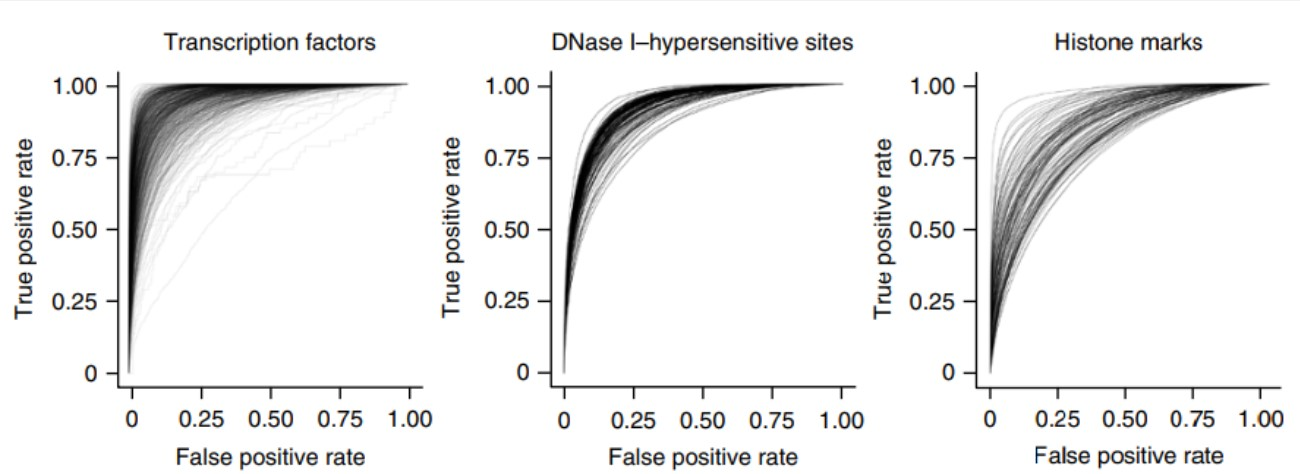
\includegraphics[width=1\textwidth]{assets/imgs/DeepSEA-AUC.jpg}   
%     \caption[DeepSEA evaluation]{DeepSEA evaluation}\label{fig:deepSEA-AUC}
% \end{figure}

\begin{comment}
Il modello è stato elaborato per predire l'effetto delle varianti non codificanti sulla cromatina. Sono presenti tre features importanti in questo modello:
\begin{enumerate}
    \item Il modello considera non solo sequenze brevi ma anche lunghe in modo da catturare informazioni più rilevanti contenute su sequenze più ampie, in modo da avere una visione ad insieme delle funzionalità
    \item Il modello riesce a apprendere pattern da diverse scale spaziali, in questo modo è possible analizzare pattern locali e globali grazie ad una struttra gerarchica (penso che sia riferita ai conv layer della CNN)
    \item Addestramento contemporaneo su diversi compiti relativi alla cromatina che condividono caratterstiche predittive. In questo modo è possibile apprendere e prevedere aspetti della cromatina.
\end{enumerate}
% 
L'articolo sottolinea l'importanza di utilizzare un contesto di sequenza più ampio perché la sequenza che circonda la posizione della variante determina le proprietà regolatorie della variante stessa e, di conseguenza, è importante per comprendere gli effetti funzionali delle varianti non codificanti: lunghezza di sequenze fino ad 1kbp

È stato poi testato il modello. Il risultato AUC per la predizione di chromatine features, tra cui TF binding sites, è stato di 0.958, superando la performance dello stato dell'arte precedente, gkm-SVM che era di 0.896. Inoltre ha ottenuto ottimi risultati anche per il DHS, con una median AUC di 0.923


\subsection*{Model Design}
Il modello presenta sequenze di conv layer e max pooling layer per estrarre man mano le features in scale spaziali diverse (capisci meglio). Alla fine cè un fully connected che permette di eleborare le informazioni e, attraverso una sgmoide, calcola la probabilità di ciascuno dei chromatine facur feature. I kerne sono le wieght matrixes. L'output di cascun conv layer è processato prima da un RElu. L'operazione di convoulzuone nel primo livello equivale a calcolare le PWM scores in un finestra, con step di 1. Nei livelli convoluzionali successivi, il kernel è una PWM sull'output del layer precedente. 
\todo{Illustra brevemente una PWM}
Nei livelli successivi al primo, il kernel è di dimension MxN, dove N è il numero di kernel utilizzati nel layer precedente. Se nel primo livello sono state utilizzate 10 PWM $12\times4$, nel lvl successivo sarà usata un kernel di dimension 12X10. Dopo il convlayer viene pushato un relu e poi u pooling: step = dimensione della pooling window.

In DeepSEA sono presenti 3 livelli convluzionali, il primo con 320 kernel, il secondo con 480 ed il terzo con 960. DOpo la convoluzione è presente un fully connected layer, dove i neuroni ricevono il risultato delle convoluzioni e fanno una relu con la matrice dei pesi che colelga 3conv-FCL (fylly conn layer)

The last layer, the sigmoid output layer, makes predictions for each of the 919 chromatin features (125 DNase features, 690 TF features, 104 histone features) and scales predictions to the 0 to 1 range by the sigmoid function

\subsection*{Model Training}
Si è definita la funzione obiettivo (cost function) come la somma del logaritmo negativo della likelihood (NLL), sommati ad altri parametri per evitare overfitting.
% 

% 
% Dove $s$ indica l'indece del sample e $f$ indica la sua feature (ovvero i vari tipo di output, che sono 919). Inoltre $y_f_s$ indica il label 0,1 rispetto alla al tipo di cromatine featre $f$ e al sample $s$. Infine $\sigma_f\left(X_s\right)$ indica il valore predetto dalla rete dato il sample $s$ sulla feture $f$.

A questa funzione vengono sommati altri attributi alla NLL al fine di evitare l'verfitting.\todo{Vedi se inserirla oppure skippare sta parte perchè è poco importante ma difficile da spiegare in quanto relies on knowledge we do not have LMAO1}
% 
\begin{gather*}
C = \mathbf{NLL} + \lambda_1\vert\vert W \vert\vert_2^2 + \lambda_2 \vert\vert H^{-1} \vert\vert_1
\end{gather*}
% 




\subsection*{Training dataset}

% , ottenuti dai progetti ``\textit{Encyclopedia of DNA Elements}'' (\acs{ENCODE}) e ``\textit{Roadmap Epigenomics}'' e

Le labels sono stte ricavate da ENCODE e Roadmap Epigenomica. Splittato il genoma in segmenti da 200bp. Per ogi frammento sono state associate le 919 chromatine features. Se più del 50\% del frammento era nella peak region della feature, era labellato a 1, altrimenti zero.

Ogni training sample consisteva nel 1000bp sequences, centrata sul frammento (bin) di 200 basi ed associata al vettore di etichette che ontiene le 919 features. In questo modo, le due sequenze di 400 bp ai lati davaano più contesto in modo da interpretare meglio il risultato.

% For evaluating performance on the test set, we used area under the receiver operating characteristic curve (AUC). The predicted probability for each sequence was computed as the average of the probability predictions for the forward and complementary sequence pairs.
\end{comment}






\section{Basset}\label{sec:Basset}
% 
Basset\footnote{Il nome richiama il bassotto, noto per le sue capacità olfattive, in analogia con l'abilità del modello di riconoscere pattern.} è un potente strumento sviluppato nel 2016, progettato per analizzare sequenze di DNA e prevedere l'accessibilità di 164 siti ipersensibili alla DNase I (\acs{DHS}), che indicano la presenza di elementi regolativi. Mediante le \acs{ConvNet}, questo modello è quindi in grado di fornire importanti informazioni rigaurdo la fase di trascrizione da \acs{DNA} ad \acs{RNA} anlizzando questi particolari siti della cromatina. Proprio come DeepSEA, la presenza di più livelli convoluzionali facilita la comprensione degli aspetti funzionali derivanti dalle mutazioni nei \acs{DHS}.

Anche Basset, come DeepSEA, è stato implementato utilizzando la libreria \href{https://github.com/torch/torch7}{\textsl{Torch7}}. Questo tool dà la possibilità di personalizzare il modello a piacimento, indicando il numero per ciascun tipo di livello, il numero di filtri (\acs{PWM}) nei livelli convoluzionali, la loro dimensione, la grandezza delle finestre di pooling, il numero di neuroni nei fully-connected layer e vari iperparametri per la fase di allenamento e di test. Attraverso l'ottimizzazione Bayesiana si sono trovati i layer e gli iperparametri ideali per l'architettura. La struttura è composta da tre livelli convoluzionali: il primo livello contiene 300 filtri di lunghezza 19bp, il secondo è composto da 200 kernel di lunghezza 11bp e il terzo layer ne contiene 200 di lunghezza 7bp. È importante sottolineare che dopo ciascun livello convoluzionale, segue un livello che normalizzi l'output della convoluzione (\textit{batch normalization}) seguito da una \acs{ReLU} ed un max-pooling layer. In seguito ai tre livelli convoluzionali sono presenti tre fully connected layer, alternati con due \acs{ReLU} e due dropout layer (con coefficiente di 0.3) che, in maniera molto simile a DeepSEA sono utilizzati per prevenire il rischio di overfitting, annullando il contributo di alcuni neuroni casuali durante l'allenamento. Infine l'output layer, attraverso la funzione sigmoide, calcola la probabilità che l'input appartenga ad uno dei 164 \acs{DHS}.

Dei siti ipersensibili alla DNasi I, 125 sono stati estratti da \acs{ENCODE} e 39 ``\textit{Roadmap Epigenomics}''. I dati estratti sono stati processati e tutti i siti sono stati isolati ed arricchiti fino ad avere un dataset iniziale di compostp da sequenze di 600bp, per un totale di $2\,071\,886$bp. Ciascuna delle sequenze presenti nel dataset sono state poi associate al vettore di label che indicava a quale dei 164 tipi la sequenza apparteneva. Dei 164 tipi, il $17\%$ dei siti sono stati associati a promoters, il $47\%$ è stato classificato come siti intragenici — ovvero all'interno dei geni — e il restante $36\%$ è stato etichettato come siti intergenici — cioè tra i geni. Infine, prima di essere utilizzati nella rete, i siti sono stati processati mediante il One-Hot encoding, formando quindi sequenze di input di dimensione $600\times 4$. Del dataset totale, $71\,886$ basi sono state utilizzate per la fase di test e altre $70\,000$ per la fase di validazione.

Il modello è stato allenato attraverso il \acs{GD} stocastico, cercando di ottimizzare la funzione binary cross entropy, il cui gradiente è stato calcolato mediante la backpropagation. Per prevenire il rischio di overfitting si è applicata la tecnica dell'\textit{early stopping}, facendo terminare l'allenamento dopo 12 epoche che la \textit{validation loss} rimane invariata. % Dopo l'allenamento e la validazione, il modello è stato testato, ottenendo un valore AUC medio di $0.895$ sui \acs{DHS}.

\begin{comment}
\subsection*{Model Design}
Weight matrixes that learn patterns. Nel livello convluzionale l'algoritmo scans le PWM (ovvero i filtri). Come nella altre CNN, durante l'allenamento i kernel imparano a riconoscere pattern importatni. IN questo modo non è ecessario specioficarliu manualmente.
% Prior work has demonstrated that with a sufficiently large data set, deep neural networks can learn far more expressive and accurate models than other common approaches like random forests or kernel methods
Dopo ogni livello convluzionale viene appliocata una relu (rectifier operation). Dopo di che viene fatto un max pooling. % This operation reduces the dimension of the input to the next layer (and thus the computation required in training).
Successivi livelli convuluzionali fanno la stessa cosa del primo. Per le sequene di DNA, i livelli usccessivi catturano interazioni spaziali con le pWM iniziali. SOno presenti 3 livelli convopluzionali (ciascuno con il recfier e la max pooling) e infine due livelli fully connected. Il livello finale pusha fuori 164 predizioni.

Sono stati utilizzati il test AUC che plotta false positive vs true popsitive graph. Come deepsea, anche basset è stato dimostrato essere piu pro di gkm-SVM

Il primo layer convoluzionale ha 300 filters. Dopo ciascun convlayer viene fatta una relu e poi una maxpool.
    
È stata usata la libreria Torch7 di python per l'implementazione.

Dopo il terzo layer convoluzionale si applica un doppoio layer fully conncted che operano una sigmoid transformation per mandare in output i 164 tipi di cellule. INltre We trained to minimize the binary cross entropy loss function, summed over these 164 outputs. Si è calcolto il gradiente della funzione obiettivo con la backpropagation.

\subsection*{Dataset}

We downloaded DNase-seq peak BED format files for 125 cell types from the ENCODE Project Consortium (2012) and 39 cell types from the Roadmap Epigenomics Consortium (2015).

Hanno fatto anche in questo caso il flanking di 600 bp: To merge the peaks into one set, we first extended each one from its midpoint to 600 bp
\end{comment}





\section{DeepSATA}\label{sec:DeepSATA}
% 
Pubblicato nel 2023, DeepSATA è il terzo tool basato su una \acs{CNN} che si occupa di identificare le \acs{OCR} — regioni aperte della cromatina — cercando di comprenderne anche la funzione. In particolare DeepSATA si concentra sulle mutazioni non codificanti nei siti di \acs{TF} binding non solo in sequenze genomiche umane, ma anche di altre specie animali quali maiali, galline, bovini e topi.

DeepSATA è un modelo basato su DeepSEA.\@ È quindi composto da tre layer convoluzionali, con rispettivamente da 320, 480 e 960 kernel (anche in questo caso rappresentati da \acs{PWM}). Ogni livello convluzionale è seguito da un layer che applica la funzione \acs{ReLU} e poi un max pooling layer estrae dal risultato le feature predominanti. Dopo ciascun livello convoluzionale è presente anche un dropout layer che, come per Basset, aiuta la rete a prevenire il rischio di overfitting. I primi due livelli di dropout hanno un coefficiente di 0.2 mentre il terzo ha un coeffciente di 0.5. Anche in questo tool, ai tre layer convoluzionali, seguono dei fully-conected layer che preparano i dati all'output layer che, attraverso la funzione sigmoide, viene calcolata la probabilita secondo il quale l'input fornito appartenga ad una tra le \acs{OCR} disponibili.

A differenza di DeepSEA, il formato della sequenza in input è tridimensionale anzichè a due dimensioni. In particolare La sequenza in input è di dimensione $M \times 4 \times (N + 1)$, dove $M$ è la lunghezza della sequenza in input e $4$ sono le basi azotate. Infine $N + 1$, ovvero la profondità della matrice tridimensionale indica le affinità specifiche che ha la sequenza di input con gli $N$ fattori di trascrizione. A questo numero si aggiunge 1, che è lo strato della codifica OneHot della sequenza. In questo modo i \acs{TF} associati alla sequenza di input aiutano a comprendere in maniera migliore gli effetti delle mutazioni nella sequenza. I \acs{TF} sono stati ottenuti dal database \textsl{JASPAR} e, mediante \textsl{FIMO}\footnote{Questo software identifica dei motif conosciuti all'interno della sequenza fornita in input.}, sono stati identificati i motif più diffusi. Di questi, sono stati selezionai i primi $N$ \acs{TF} più presenti da inserire nel dataset iniziale. Per motivi legati alle risorse disponibili, gli autori dell'articolo hanno scelto $N=10$ siti di legame dei \acs{TF}. 

Il dataset che contiene sequenze di più specie è stato raccolto rispettivamente dai seguenti database:
\begin{itemize}
    \item Le sequenze relative ai topi sono state ottenute dall'\textit{\acs{NCBI} Sequence Read Archive} (\acs{SRA});
    \item I tratti di genoma unamo sono stati ricavati da \acs{ENCODE};
    \item Le sequenze genomiche dei maili sono state ottenute dal \textit{Gene Expression Omnibus} (\acs{GEO});
    \item Le porzioni di \acs{DNA} relative a bovini e polli sono state scaricate dal sito dell'Università della California (\textsl{UC Davis}), nella sezione \textit{Farm Clusters}.
\end{itemize} 
% 
\noindent Dopo aver raccolto tutti i dati necessari, in maniera del tutto analoga a DeepSEA, sono stati divisi in bin da 200bp ed etichettati a seconda della \acs{OCR} che rappresentavano: se più della metà della sequenza aveva una corrispondenza con una \acs{OCR}, veniva impostata l'etichetta ad 1 per quella particolare regione della cromatina, altrimenti 0. In secondo luogo, sono stati centrati con sequenze lunghe 400bp per avere sequenze di 1000bp come input, chiamate anche \textit{Open Chromatin Bin} (\acs{OCB}). Di conseguenza, ciascun bin di input, una volta effettuato il OneHot encoding è rappresentato da una matrice di dimensione $1000 \times 4 \times 11$.

Essendo DeepSATA un modello basato su DeepSEA, il modelli è stato allenato attraverso il \acs{GD} stocastico con momento per ottimizzare la funzione di binary cross entropy. In maniera del tutto analoga, il gradiente di questa funzione è stato calcolato mediante l'algoritmo della backpropagation

% 
\begin{comment}

DeepSATA è uno framework user-friendly, progettato per identificare le regioni aprte di cromatina (OCR) lungo l'intero genoma e le functional annotation delle varianti non codificanti (con annotazione funzionale si intende il processo di descrivere la struttura e la funzione di un componente del genoma).

Il modello è composto da 3 layer, con 320, 480 e 960, ciascuno dei quali seguito da una relu, max pooling e dropout. E applicata la sigmoide per per generare gli output, ovvero la probabilita per la cromatina. Vengono citati ancora una volta i 200 bins flankati di 400 a dtesta e sinistra per dare contesto. Ogni sequenza in input era tridimensionale. Ricordiamo che la terza dimensione, N + 1, rappresenta le configurazioni di legame dei fattori di trascrizione (TF). In particolare, il primo strato in questa dimensione è la codifica one-hot della sequenza di DNA stessa, mentre i successivi strati (dallo strato 2 allo strato N + 1) codificano le affinità di legame e le posizioni specifiche di ciascun TF. Questo approccio consente al modello di considerare non solo la composizione della sequenza ma anche come diversi TF interagiscono con essa, fornendo un contesto ricco e complesso per l'analisi della regolazione genica.

I dati relativi alle specie, sono stati presi dai seguenti databasse:
\begin{itemize}
    \item Topi, e NCBI Sequence Read Archive (SRA)
    \item Umani, ENCODE
    \item SPecie dei Maiali deiravta da e Gene Expression Omnibus (GEO)
    \item Bovini e polli sono stati prelevati dal sito del UC-DAVi university, californi, Farm Clusters
\end{itemize} 

Per le sequenze di DNA, deepsata estende la matrice bidimensionale che rappresenta la sequenza genomica dopo il onehot encoding (matrice M X 4) in una matrice tridimensionale che incorpora anche le binding configuration dei TFs che sono importanti per capire il contesto di studio. Questi TFs sono selezionati per arricchire il dna bionding motif con le OCR, regioni aperte di cromatina. In seguito, lungo la terza dimensione della matrice, ciascun layer convoluzionale successivo codifica l'affinità di legame (biding) dimension un fattore di trascrizione specifico. La strategia di codifica consiste nell'utilizzare la matrice di probabilità dei pesi di posizione del fattore di trascrizione (TF) per popolare la matrice nel suo sito di legame previsto.

Il genoma è stato diviso in bin da 200bp. Ad ogni bin è stata assegnata l'etichetta 0 o 1 se almeno meta dei 200 bp confomavano alla ATAC peak region. Ogni OCB (Open chromatin bins), associato ai sui 400bp di flanking sequence è stato poin buttato dentro deppsata. Ogni OCB è composto dalla strattura $1000 \times 4 \times (N + 1)$, dove N sono i TFs che sono stati predictati legare la sequenza. Per determinare N nel training set sono statti collezionait TF binding sites da Jaspar 2022 database e poi è stato usato FIMO 5.4.1 per identificare la presenza dei motivbi. Dopo di che i TF sono stati rankati i primi N TFS per l'allenamento del modello. Nell'articolo viene indicato che si è deciso di inserire N = 10 a causa di resource constraints.

Copo ciascun layer convoluzionale, viene effettuata una ReLu legegrmente modificata: per evitare gli overfitting, i pesi sono stati messi a 0.000001 quando minori di zero. In seguito alla ReLu viene fatta una maxpooling di grandezza 4 X N + 1, per combinare le feature che sono state estratte dai vari OCB types. Infine, dopo la max pooling viene effettuato un droput con rate di 0.2 per evitare overfitting e rendere a rete pi robusta. Per i livelkli convoluzionali seguenti sono stati utilizzati 480 e 960 kernel. I parametri della ReLu activatioon erano gfli stessi del primo layer. Per quanto riguarda la max pooling, ha size $4 \times 1$, per cionsentire il downsampling del dataset e graantire un miglior traingin experince trolp letsgoski. In questo caso il droput rate è stato butatto a 0.2 e 0.5, per prevenire l'overfitting.
\end{comment}

    %!TEX root = ../main.tex

\chapter{Discussione}\label{chp:discussion}


Dopo aver dettagliatamente descritto le caratterstiche dei tre strumenti bioinformatici nel Capitolo\,\ref{chp:CNN-non-coding-variants}, in questo capitolo si paragoneranno i tre tool, sottolineando le proprietà comuni e gli aspetti per cui differiscono in modo da fornire un confornto oggettivo che permette di comprendere in maniera più approfondita le loro performance predittive.

DeepSEA, Basset e DeepSATA, hanno alcune caratterstiche in comune. I tre tool utilizzano lo stesso metodo di codifica della sequenza, il One-Hot encoding, che rende la sequenza luna $M$ in una matrice $M\times 4$, mappando le basi azotate della sequenza in vettori. Più precisamente, la codifica scelta è stata quella di codificare le basi azotate come segue: $A \to \left[1, 0, 0, 0\right]$, $T \to \left[0, 1, 0, 0\right]$, $C \to \left[0, 0, 1, 0\right]$ e $G \to \left[0, 0, 0, 1\right]$. In questo modo la sequenza può essere processata correttamente dai kernel, che sono delle \acs{PWM} che associano a ciascuna base delle sequenza un peso (o probabilità di occorrenza) in una particolare posizione (Figura\,\ref{fig:PWM}). Infine i tre modelli sono stati allenati attraverso il \acs{SGD} cercando di ottimizzare la stessa funzione obiettivo (cost function): la binary cross entropy (\acs{BCE}).

Nonstante le similarità descritte, i tre strumenti prensentano diverse differenze, soprattutto nella struttura della rete e nel training dataset scelto: la Tabella\,\ref{tab:summary} riassume le caratteristiche principali. \,\hyperref[sec:DeepSEA]{\textsl{DeepSEA}} è composto da tre livelli convoluzionali, ciascuno dei quali viene seguito sempre da un livello \acs{ReLU} e da un livello max-pooling, utilizzato per estrarre le feature dominanti processate dalla convoluzione. I tre livelli convoluzionali contengono rispettivamente 320, 480 e 960 filtri. In seguito è presente un fully-conncted layer che prepara la informazioni per essere valutate nell'output layer, formato da una sigmoide.

Anche \hyperref[sec:Basset]{\textsl{Basset}} è composto da tre livelli convoluzionali ma in aggiunga al \acs{ReLU} layer e al max-pooling layer viene inserito anche un livello di normalizzazione. Sono poi presenti tre livelli fully-connected che sono alternati da altri \acs{ReLU} layer e dei dropout layer, per evitare l'overfitting. Anche in questo caso l'output è calcolato tramite una sigmoide.
% 
\begin{table}[!t]
    \centering
    \caption{Riassunto delle differenza tra i tre tool.}\label{tab:summary}
    \renewcommand{\arraystretch}{2}
    \begin{tabular}{|>{\centering\arraybackslash}m{2cm}|>{\centering\arraybackslash}m{4.5cm}|>{\centering\arraybackslash}m{1.5cm}|>{\centering\arraybackslash}m{1.5cm}|>{\centering\arraybackslash}m{3cm}|} % chktex-file 44
        \hline % chktex-file 44
        \textbf{Modello} & \textbf{Struttura} & \textbf{Kernel} & \textbf{Input} & \textbf{Dataset} \\ 
        \hline\hline % chktex-file 44
        \hyperref[sec:DeepSEA]{\textsl{DeepSEA}} & Tre livelli convoluzionali — ciascuno seguito da un \acs{ReLU} layer e da un max-pooling layer — e un fully-connected layer  &  320, 480, 960 & $1000\times 4$ & \acs{ENCODE}, Roadmap Epigenomics\\ 
        % 
        \hyperref[sec:Basset]{\textsl{Basset}} & Tre livelli convoluzionali — ciascuno seguito da un normalization layer, un \acs{ReLU} layer e da un max-pooling layer — e tre fully-connected layer — alternati da un \acs{ReLU} layer ed un dropout layer &  300, 200, 200 & $600 \times 4$ & \acs{ENCODE}, Roadmap Epigenomics\\ 
        % 
        \hyperref[sec:DeepSATA]{\textsl{DeepSATA}} & Tre livelli convoluzionali — ciascuno seguito da un \acs{ReLU} layer, da un max-pooling layer e da un dropout layer — e un fully-connected layer & 320, 480, 960 & $1000\times 4\times 11$ & \acs{ENCODE}, \acs{NCBI} \acs{SRA}, \acs{GEO}, UC Davis\\ 
        \hline
    \end{tabular}
    \renewcommand{\arraystretch}{1}
\end{table}

Come DeepSEA e Basset, anche \hyperref[sec:DeepSATA]{\textsl{DeepSATA}} è composto da tre livelli di convoluzione, con rispettivamente 320, 480 e 960 kernel. Ad ogni layer convoluzionale segue un \acs{ReLU} layer, un max-pooling layer ed un dropout layer, per prevenire il rischio di overfitting. Ai livelli convoluzionali segue un fully connected layer che processa le informazioni per l'output layer che applica una funzione sigmoide. Si osserva inoltre che in questo modello, a differenza degli altri due, processa un input tridimensionale, volto a fornire più contesto per comprendere in maniera migliore gli eventuali effetti delle mutazioni sulla sequenza.

Gli autori dell'articolo che introduce DeepSATA, dopo aver illustrato il modello e le principali differenza con il suo predecessore DeepSEA, conducono un esperimento dove paragonano le capacità predittive di DeepSEA, Basset e DeepSATA.\@ In particolare, dopo aver allenato i tre modelli sul dataset contenente sequenze di specie animali diverse, tra cui l'uomo, valutano le prestazione dei modelli. Dai risultati del test (Tabella\,\ref{tab:comparison}) si nota che le prestazioni predittive di DeepSATA, anche se non di molto, superano le prestazioni di DeepSEA e di Basset. In particolare si nota una maggiore differenza nelle sequenze genetiche dei maiali, dove il valore \acs{AUC}/\acs{AUROC} è superiore di più di cinque punti percentuale. Nelle altre specie invece, anche se non di tanto, DeepSATA ottiene comunque risultati migliori.
\begin{table}[!h]
    \centering
    \caption{Riassunto del confronto tra DeepSEA, Basset e DeepSATA}\label{tab:comparison}
    \renewcommand{\arraystretch}{2}
    \begin{tabular}{|>{\centering\arraybackslash}p{2cm}|>{\centering\arraybackslash}p{2cm}|>{\centering\arraybackslash}p{2cm}|>{\centering\arraybackslash}p{2cm}|>{\centering\arraybackslash}p{2cm}|>{\centering\arraybackslash}p{2cm}|} % chktex-file 44
        \hline % chktex-file 44
        \textbf{Modello} & \textbf{Topi} & \textbf{Maiali} & \textbf{Bovini} & \textbf{Umani} & \textbf{Polli}\\ 
        \hline\hline % chktex-file 44
        \hyperref[sec:DeepSATA]{\textsl{DeepSATA}} & 0.854 & 0.779 & 0.772 & 0.759 & 0.744 \\ 
        % 
        \hyperref[sec:DeepSEA]{\textsl{DeepSEA}} & 0.796 & 0.775 & 0.769 & 0.755 & 0.736 \\ 
        % 
        \hyperref[sec:Basset]{\textsl{Basset}} & 0.778 & 0.719 & 0.768 & 0.717 & 0.722 \\ 
        \hline
    \end{tabular}
    \renewcommand{\arraystretch}{1}
\end{table}
Dalla Tabella\,\ref{tab:comparison} si nota che i valori \acs{AUROC} di DeepSATA e DeepSEA differiscono di pochi  millesimi tra loro, a differenza dei valori di Basset, che talvolta sono nettamente più bassi rispetto ai valori degli altri due modelli. In particolare sulle sequenze che riguardano il genoma umano si nota una differenza di circa quattro punti percentuale tra Basset e DeepSEA/DeepSATA.\@
% 
\begin{figure}[!b]
    \centering
    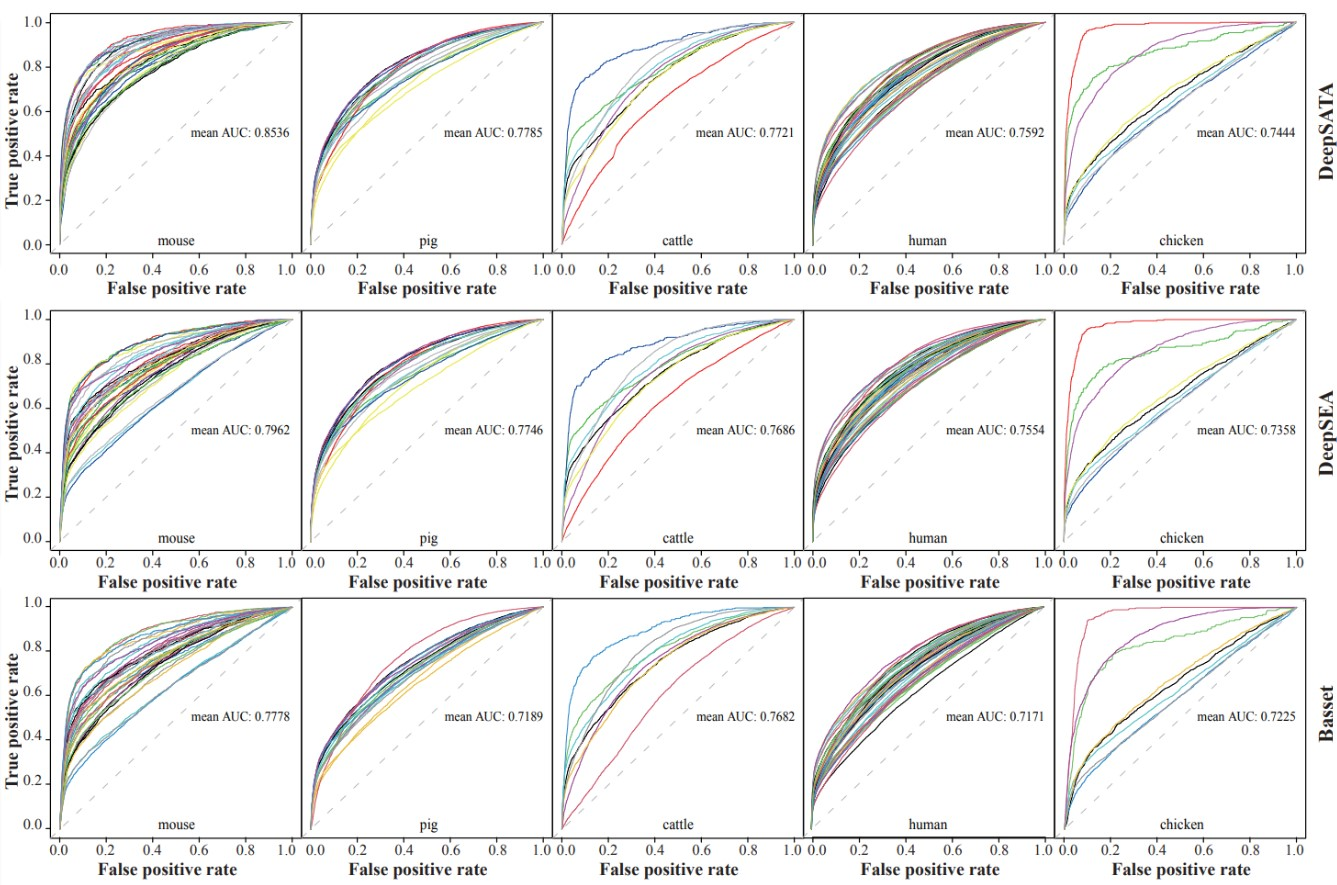
\includegraphics[width=1\textwidth]{assets/imgs/comparison.jpg}
    \caption[Confronto delle prestazioni predittive dei tre tool su diverse specie animali.]{Confronto delle prestazioni predittive dei tre tool su diverse specie animali\,\cite{ma2023deepsata}.}\label{fig:comparison}
\end{figure}
% 
Di conseguenza, la tabella, oltre che ad indicare che DeepSATA abbia capacità predittive migliori rispetto agli altri due strumenti, suggerisce che il modello di DeepSEA riesce a riconoscere in maniera migliore le categorie rispetto a Basset. Le informazioni riportate sulla Tabella\,\ref{tab:comparison} sono anche rappresentate sotto forma di curve \acs{ROC} nella Figura\,\ref{fig:comparison}, dove sono indicate le performance predittive di ciascun modello a seconda delle specie animali in esame.

\begin{comment}
    In our study, we utilized DeepSATA to evaluate its predictive capabilities for chromatin features in five distinct species: mice, pigs, cattle, humans, and chickens. We collected open chromatin accessibility datasets and corresponding transcription factor binding motifs, which are summarized in Table 1 and Supplementary Tables S1 and S2. The performance of the DeepSATA, DeepSEA, and Basset models was assessed for each species by comparing their average AUC values across different chromatin features. DeepSATA demonstrated superior performance across all species, with average AUC values of 0.854, 0.779, 0.772, 0.759, and 0.744 for mice, pigs, cattle, humans, and chickens, respectively (Figure 2A and Supplementary Table S3). In comparison, DeepSEA had average AUC values of 0.796, 0.775, 0.769, 0.755, and 0.736, respectively (Figure 2B and Supplementary Table S3), while Basset had average AUC values of 0.778, 0.719, 0.768, 0.717, and 0.722, respectively (Figure 2C and Supplementary Table S3). It is worth noting that DeepSATA consistently outperformed DeepSEA and Basset in all chromatin features for pigs and mice (Supplementary Table S3). The relative improvement was particularly significant in the cerebrum tissue of the mice, where DeepSATA achieved an AUC of 0.829 compared to DeepSEA’s 0.659 for female mice and an AUC of 0.828 compared to DeepSEA’s 0.653 for male mice, representing a relative improvement of over 25%. Interestingly, our findings indicate that the DeepSATA, DeepSEA, and Basset models performed better for the Duroc pig breed compared to other pig breeds (Supplementary Table S3). This suggests a superior ability to recognize regulatory functional patterns in the non-coding genomic regions  pecific to Duroc pigs. In the case of cattle, the chromatin feature of the hypothalamus was most effectively captured, with AUC values of 0.887 for DeepSATA, 0.883 for DeepSEA, and 0.895 for Basset (Supplementary Table S3). What particularly encouraged us was the remarkable performance of DeepSATA in accurately recognizing the regulatory patterns of the cerebellum in chickens, achieving AUC values as high as 0.972, while DeepSEA achieved 0.971 and Basset achieved 0.953 (Supplementary Table S3). Additionally, in the following analysis, we selected DeepSEA as the baseline comparison, since it achieved better prediction performance compared with Basset. Overall, these results clearly demonstrate the effectiveness of DeepSATA in accurately identifying the regulatory patterns of chromatin features in different animal species
\end{comment}

    %!TEX root = ../main.tex

\chapter{Conclusioni}\label{chp:conclusions}

    
    % Bibliography, appendix, acknowledges, etc...
    \backmatter
\end{document}
